% Manuscript preprint — hand-curated LaTeX, tectonic-built (ticket 0524).
% Converted from the former pandoc/pandoc-crossref main.md (one-shot
% `pandoc -t latex` starting point, then curated). This file is the source
% of truth; build with `make -C slides manuscript/main.pdf`.
%
% Conventions (see .claude/rules/writing.md):
% - Cross-references are symbolic: \label / \ref, never hand-typed numbers.
%   Section refs render as §N via the literal prefix `§\ref{...}`; figure and
%   table refs as `Figure~\ref{...}` / `Table~\ref{...}`. Annex refs use bare
%   \ref — \appendix redefines \thesection to "Annex A" lettering.
% - Figures are committed PDF artifacts under report/inputs/generated/,
%   included by \includegraphics. Paths are relative to this file's directory
%   (tectonic resolves against the input file's location): ../../report/...
\documentclass[a4paper,11pt]{article}

% Fonts (XeTeX/Tectonic)
\usepackage{fontspec}
\usepackage{amsmath}
\defaultfontfeatures{Ligatures=TeX}

% Typography
\usepackage{microtype}
\usepackage{parskip}
\setlength{\emergencystretch}{3em}
\setcounter{secnumdepth}{3}
\providecommand{\tightlist}{%
  \setlength{\itemsep}{0pt}\setlength{\parskip}{0pt}}

% Glyphs absent from Latin Modern text fonts
\usepackage{newunicodechar}
\newunicodechar{✕}{\ensuremath{\times}}
\newunicodechar{≤}{\ensuremath{\leq}}
\newunicodechar{≥}{\ensuremath{\geq}}
\newunicodechar{≈}{\ensuremath{\approx}}
\newunicodechar{ρ}{\ensuremath{\rho}}
\newunicodechar{τ}{\ensuremath{\tau}}
\newunicodechar{Δ}{\ensuremath{\Delta}}
\newunicodechar{−}{\ensuremath{-}}
\newunicodechar{⁴}{\ensuremath{^{4}}}
\newunicodechar{→}{\ensuremath{\rightarrow}}
\newunicodechar{↔}{\ensuremath{\leftrightarrow}}
\newunicodechar{·}{\ensuremath{\cdot}}

% Tables and figures
\usepackage{longtable,booktabs,array}
\usepackage{graphicx}
\usepackage{pdfpages} % \includepdf: multi-page portrait recognition matrix
\usepackage{xcolor}

% Bibliography
\usepackage[round,authoryear]{natbib}
\bibliographystyle{plainnat}

% Consolidated manuscript macros (ticket 0531): every empirical number the
% prose quotes is a \newcommand generated by the pipeline (Makefile-wired,
% regenerated by `make -f experiments/render.mk report-tables`). The explicit
% relative path defuses the tectonic bundle trap (.claude/rules/writing.md).
% Consolidated manuscript macros — generated by experiments/render.mk (ticket 0531).
% DO NOT EDIT — concatenation of the per-script fragments in MANUSCRIPT_MACRO_FRAGMENTS.
% Regenerate with: make -f experiments/render.mk report-tables
% Auto-generated by aedist.analyze_matcher_phase_collisions — do not edit.
\newcommand{\PhaseCollisionPairsNinety}{174}
\newcommand{\PhaseCollisionVetoBlockedNinety}{104}
\newcommand{\PhaseCollisionResidualNinety}{70}
\newcommand{\PhaseCollisionPairsEightyFive}{195}
\newcommand{\PhaseCollisionPairsNinetyFive}{94}
\newcommand{\RealisedFuzzyBelowNinety}{0}
% Mean-F1 drop from threshold 90 to 95, averaged over the 195 runs at each threshold in matching_sensitivity.csv; not yet cited in the manuscript — defined for future citation.
\newcommand{\ThresholdSensFOneDropNinetyFive}{0.046}
% Auto-generated by aedist.tabulate_exp1_run_stats — do not edit.
\newcommand{\ExpOneFOneMin}{0.00}
\newcommand{\ExpOneFOneMean}{0.38}
\newcommand{\ExpOneFOneMax}{0.68}
\newcommand{\ExpOneNRuns}{70}
\newcommand{\ExpOneNModels}{14}
\newcommand{\ExpOneFuelAcc}{0.54}
\newcommand{\ExpOneStatusAcc}{0.57}
\newcommand{\ExpOneProvinceAcc}{0.89}
% Auto-generated by aedist.plot_exp1_matrix — do not edit.
\newcommand{\ExpOneMatrixPlants}{177}
\newcommand{\ExpOneMatrixRuns}{70}
\newcommand{\ExpOneMatrixFPs}{40}
% Auto-generated by aedist.plot_exp1_matrix — do not edit.
\newcommand{\ExpTwoNaiveMatrixPlants}{177}
\newcommand{\ExpTwoNaiveMatrixRuns}{20}
\newcommand{\ExpTwoNaiveMatrixFPs}{33}
% Auto-generated by aedist.plot_exp1_matrix — do not edit.
\newcommand{\ExpTwoOptMatrixPlants}{177}
\newcommand{\ExpTwoOptMatrixRuns}{20}
\newcommand{\ExpTwoOptMatrixFPs}{25}
% Auto-generated by aedist.plot_exp1_matrix — do not edit.
\newcommand{\ExpTwoArmThreeMatrixPlants}{177}
\newcommand{\ExpTwoArmThreeMatrixRuns}{20}
\newcommand{\ExpTwoArmThreeMatrixFPs}{40}
% Auto-generated by aedist.plot_exp1_matrix — do not edit.
\newcommand{\ExpTwoArmFourMatrixPlants}{177}
\newcommand{\ExpTwoArmFourMatrixRuns}{20}
\newcommand{\ExpTwoArmFourMatrixFPs}{40}
% Auto-generated by aedist.plot_method_convergence — do not edit
\newcommand{\NumCensusModels}{14}
\newcommand{\CensusTPMin}{0}
\newcommand{\CensusTPMax}{116}
\newcommand{\CensusFPMin}{0}
\newcommand{\CensusFPMax}{484}
\newcommand{\CensusNumRuns}{70}
\newcommand{\CensusNumOk}{70}
\newcommand{\CensusNumRefusal}{0}
\newcommand{\CensusCostTotal}{6.21}
\newcommand{\CensusCostMin}{0.0006}
\newcommand{\CensusCostMax}{0.4709}
\newcommand{\CensusWallMin}{18}
\newcommand{\CensusWallMax}{1200}
% Fusion MVP macros — generated by aedist.plot_fusion_mvp
% DO NOT EDIT — regenerate with: make -f experiments/render.mk fusion-mvp

% Regime: E1
\newcommand{\FusionNEOneRuns}{20}
\newcommand{\FusionNEOneModels}{4}
\newcommand{\FusionBestEOneF}{66.6\%}
\newcommand{\FusionBestEOneRecall}{51.2\%}
\newcommand{\FusionBestEOnePrec}{95.5\%}
\newcommand{\FusionBestEOneFFrac}{0.666}
\newcommand{\FusionBestEOneRecallFrac}{0.512}
\newcommand{\FusionBestEOnePrecFrac}{0.955}
\newcommand{\FusionBestEOneTP}{91}
\newcommand{\FusionBestEOneFP}{4}
\newcommand{\FusionUnionEOneF}{74.1\%}
\newcommand{\FusionUnionEOneRecall}{71.2\%}
\newcommand{\FusionUnionEOnePrec}{77.3\%}
\newcommand{\FusionUnionEOneFFrac}{0.741}
\newcommand{\FusionUnionEOneRecallFrac}{0.712}
\newcommand{\FusionUnionEOnePrecFrac}{0.773}
\newcommand{\FusionUnionEOneTP}{126}
\newcommand{\FusionUnionEOneFP}{37}
\newcommand{\FusionRTwoEOneF}{75.4\%}
\newcommand{\FusionRTwoEOneRecall}{60.5\%}
\newcommand{\FusionRTwoEOnePrec}{100.0\%}
\newcommand{\FusionRTwoEOneFFrac}{0.754}
\newcommand{\FusionRTwoEOneRecallFrac}{0.605}
\newcommand{\FusionRTwoEOnePrecFrac}{1.000}
\newcommand{\FusionRTwoEOneTP}{107}
\newcommand{\FusionRTwoEOneFP}{0}

% Regime: E2-1D
\newcommand{\FusionNETwoOneDRuns}{20}
\newcommand{\FusionNETwoOneDModels}{4}
\newcommand{\FusionBestETwoOneDF}{77.5\%}
\newcommand{\FusionBestETwoOneDRecall}{67.2\%}
\newcommand{\FusionBestETwoOneDPrec}{92.4\%}
\newcommand{\FusionBestETwoOneDFFrac}{0.775}
\newcommand{\FusionBestETwoOneDRecallFrac}{0.672}
\newcommand{\FusionBestETwoOneDPrecFrac}{0.924}
\newcommand{\FusionBestETwoOneDTP}{119}
\newcommand{\FusionBestETwoOneDFP}{10}
\newcommand{\FusionUnionETwoOneDF}{76.4\%}
\newcommand{\FusionUnionETwoOneDRecall}{87.6\%}
\newcommand{\FusionUnionETwoOneDPrec}{67.7\%}
\newcommand{\FusionUnionETwoOneDFFrac}{0.764}
\newcommand{\FusionUnionETwoOneDRecallFrac}{0.876}
\newcommand{\FusionUnionETwoOneDPrecFrac}{0.677}
\newcommand{\FusionUnionETwoOneDTP}{155}
\newcommand{\FusionUnionETwoOneDFP}{74}
\newcommand{\FusionRTwoETwoOneDF}{81.3\%}
\newcommand{\FusionRTwoETwoOneDRecall}{70.1\%}
\newcommand{\FusionRTwoETwoOneDPrec}{96.9\%}
\newcommand{\FusionRTwoETwoOneDFFrac}{0.813}
\newcommand{\FusionRTwoETwoOneDRecallFrac}{0.701}
\newcommand{\FusionRTwoETwoOneDPrecFrac}{0.969}
\newcommand{\FusionRTwoETwoOneDTP}{124}
\newcommand{\FusionRTwoETwoOneDFP}{4}
% Auto-generated by aedist.plot_longtail_recognition — do not edit.
\newcommand{\LongtailReference}{177}
\newcommand{\LongtailGem}{157}
\newcommand{\LongtailWiki}{130}
\newcommand{\LongtailOsm}{49}
% Auto-generated by aedist.tabulate_source_concordance — do not edit.
\newcommand{\GemDistinct}{119}
\newcommand{\GemReviewed}{157}
\newcommand{\GemReviewedPct}{89}
\newcommand{\GemOnly}{12}
\newcommand{\WikiReviewed}{130}
\newcommand{\WikiReviewedPct}{73}
% Auto-generated by audit_exp2_wiki_citations.py — do not edit.
\newcommand{\ExpTwoWikiRunsScanned}{40}
\newcommand{\ExpTwoWikiBannedOptimised}{5}
\newcommand{\ExpTwoWikiBannedNaive}{1}
\newcommand{\ExpTwoWikiBannedTotal}{30}
% Auto-generated by aedist.screen_validation_within_model — do not edit.
\newcommand{\ScreenTauCap}{0.321}
\newcommand{\ScreenTauCapConcordant}{70}
\newcommand{\ScreenTauCapDiscordant}{36}
\newcommand{\ScreenTauStatus}{0.419}
\newcommand{\ScreenTauStatusConcordant}{66}
\newcommand{\ScreenTauStatusDiscordant}{27}
\newcommand{\ScreenPositiveSpearman}{11}
\newcommand{\ScreenNModels}{14}
\newcommand{\ScreenNMixed}{3}
\newcommand{\ScreenPooledVetoedMeanFOne}{0.150}
\newcommand{\ScreenPooledSurvivingMeanFOne}{0.491}
\newcommand{\ScreenPooledGap}{0.341}
\newcommand{\ScreenBinaryGap}{0.190}
\newcommand{\ScreenVetoedMeanFOne}{0.112}
\newcommand{\ScreenSurvivingMeanFOne}{0.350}
\newcommand{\ScreenPerModelGaps}{deepseek-v4-flash: +0.378, gpt-oss-120b: +0.077, qwen3.6-flash: +0.116}
\newcommand{\ScreenFalseVetoModel}{qwen3.6-flash}
\newcommand{\ScreenFalseVetoRun}{1}
\newcommand{\ScreenFalseVetoFOne}{0.208}
% Auto-generated by aedist.tabulate_status_difficulty — do not edit
\newcommand{\StatusProposedCount}{68}
\newcommand{\StatusProposedSharePct}{38.4}
\newcommand{\StatusProposedRatePct}{8.1}
\newcommand{\StatusOverallRatePct}{26.6}
\newcommand{\ExpOneStatusAccExclProposed}{0.62}
% Auto-generated by aedist.tabulate_aggregation_sweep — do not edit.
\newcommand{\AggBestUnionRecall}{0.644}
\newcommand{\AggBestUnionCost}{0.94}
\newcommand{\AggBestUnionCandidates}{166}
\newcommand{\AggBestUnionFOne}{0.665}
\newcommand{\AggSingleRunMeanRecall}{0.266}
\newcommand{\AggUnionGainX}{2.4}
\newcommand{\AggBestSingleRecall}{0.672}
\newcommand{\AggBestSingleFOne}{0.679}
\newcommand{\AggIntraPoolThreeRecall}{0.397}
\newcommand{\AggIntraPoolThreeCost}{0.25}
\newcommand{\AggLowRecallMin}{0.26}
\newcommand{\AggLowRecallMax}{0.42}
% Auto-generated by aedist.tabulate_reference_macros — do not edit.
\newcommand{\NumRefPlants}{177}
\newcommand{\RefCoalCount}{85}
\newcommand{\RefGasOilCount}{92}


% Links
\usepackage{bookmark}
\usepackage{xurl}
\urlstyle{same}
\hypersetup{
  pdftitle={Can Frontier AI Build a Statistical Register? A Benchmark and Research Programme on Vietnam's Thermal Power Fleet},
  hidelinks}

\title{Can Frontier AI Build a Statistical Register?\\
A Benchmark and Research Programme on Vietnam's Thermal Power
Fleet\thanks{Technical report accompanying a talk at Econom'IA 2026, Paris.
Original talk title: Beyond RAG: Stateful-Agentic Architectures for Reliable
Economic Statistics.}}
\author{Minh Ha-Duong\\
\href{https://orcid.org/0000-0001-9988-2100}{ORCID 0000-0001-9988-2100}
--- \href{mailto:minh.ha-duong@cnrs.fr}{\nolinkurl{minh.ha-duong@cnrs.fr}}\\
CIRED --- Centre International de Recherche\\
sur l'Environnement et le Développement, CNRS, France}
\date{\today}

\begin{document}

\maketitle

\begin{abstract}
Open energy-system models need plant-level data that
are complete, dated, and traceable to sources, yet across much of the
world these data arrive late or incomplete.
We introduce a computable benchmark for this task: reconstruct the
register of Vietnam's \NumRefPlants{} thermal power plants and score the result
against a hand-compiled, fully sourced reference. The register spans the
whole project lifecycle: proposed and planned projects as well as
operating, cancelled, and retired plants. The task is hard for today's
AI systems. Fourteen language models answering from memory recover at
most about two thirds of the plants, and usually far fewer, even though
group-seeded Wikipedia lists covering 92\% of the built fleet had sat in
their training corpus for years. Four frontier agents with web access
and extended reasoning improve coverage, but they still fall short on
the quality dimensions measured here: row-level accuracy, coverage, and
citation-based provenance. The experiments point toward a working
hypothesis about why: the binding constraint is the quality of the
source documents, not the capability of the model. In an exploratory,
unregistered condition, handing the agents a curated document set in a
single query equalised three of the four; the multi-turn protocol did
not replicate the effect. Finally, reference-free coherence criteria
suffice to screen out the weakest models: degenerate outputs betray
themselves by template-like, near-constant tables, so the worst runs can
be rejected without any ground truth. The results argue for investing in
the corpus and the sourcing process rather than in a stronger model,
building a sourced, auditable knowledge base from which statistical
tables derive as dated snapshots.
\end{abstract}

\section{Introduction}\label{sec:intro}

Open energy-system models such as PyPSA-ASEAN
\citep{PyPSAmeetsEarth2025:pypsa-asean} need power-plant
inventories that are complete, accurately dated, and traceable to
primary sources --- the data infrastructure for quasi-real-time policy
analysis in countries where the energy system changes faster than
publication cycles. Yet across most of the world the relevant facts
arrive late, incomplete, or under licences that forbid redistribution,
even though the underlying information is already public --- scattered
across project documents, master plans, environmental assessments,
operator reports, and press releases. The general problem behind the
specific one is older than AI: science needs knowledge, not opinions.
Statistical work requires facts that are sourced, reproducible, and
auditable, not fluent output from a plausible-text generator somewhere
in the cloud.

This paper addresses a concrete task, building a complete, sourced
inventory of Vietnam's thermal power plants, as a lens for evaluating
whether AI systems can yet produce research-grade statistical data.
Computable benchmarks, tasks whose success criteria a machine can check,
are how knowledge engineering and AI research have long measured
progress, from knowledge-base construction with language models
\citep{Petroni-Fabio2019:lm-as-kb, Singhania-Sneha2022:lm-kbc} to the
benchmark suites that rank today's systems \citep{Hendrycks-Dan2021:mmlu,
Ni-Shiwen2025:llm-benchmark-survey}; this paper extends the practice to
national statistical registers. Three results stand out. First, we offer
a new computable benchmark, scored against a hand-compiled, fully
sourced reference. We use \emph{benchmark} in the narrow sense of a
frozen task definition, a public gold reference, and a computable
metric --- not a suite or a leaderboard --- and the design measures
training-data contamination, as a parametric ceiling, rather than
trying to prevent it. Second, the task is hard for today's agents: neither
model memory nor web access yields a complete, well-sourced register.
Third, reference-free coherence criteria suffice to screen out the
weakest models.

\textbf{Contributions.} This paper makes three contributions.

\begin{itemize}
\tightlist
\item
  \emph{Benchmark gap.} To our knowledge, the first sourced evaluation
  of AI agents on national power-plant inventory construction, scored
  against a held-out reference, with per-row citation coverage and
  corroboration measured (the paper counts and checks the presence of
  citations; it does not verify each cited source against each cell).
\item
  \emph{Per-row provenance × temporality scoring.} A four-dimension
  quality bar (accuracy, coherence, provenance, temporality) applied to
  LLM-generated statistical tables.
\item
  \emph{Two-grain credibility/reliability scoring.} A run-level
  credibility screen and a model-level reliability grade, by analogy
  with the NATO Admiralty grading of STANAG 2511 (run-level information
  credibility versus model-level source reliability).
\end{itemize}

We situate the work against the existing open
power-plant databases (§\ref{sec:related-empirical}), define a
four-dimensional quality bar (§\ref{sec:quality}), survey AI
capabilities from chatbots to agentic systems (§\ref{sec:capability}),
measure what model memory alone delivers across 14 language models
(§\ref{sec:exp1}), test the commercial frontier of mid-2026
(§\ref{sec:exp2}), and show that targeted pipeline design is needed to
bridge the gap (§\ref{sec:fusion}). The Discussion
(§\ref{sec:discussion}) examines why a single aggregate score cannot
certify fitness for use and prefigures a fusion-based research
programme.

\section{Related Work --- Empirical landscape}\label{sec:related-empirical}

\textbf{Open power-plant databases.} Credible open-source energy
modelling depends on trustworthy plant-level inventories. PyPSA
\citep{Brown-Tom2018:pypsa} and its global extension PyPSA-Earth
\citep{Parzen-Maximilian2023:pypsa-earth} formalise the demand:
scenarios require asset-level data --- capacity, fuel, status, vintage
--- that is machine-readable, versioned, and traceable. The principal
public inventories are the World Resources Institute Global Power Plant
Database \citep{Byers-Logan2018:wri-gppd} and the Global Energy Monitor
Coal Plant Tracker \citep{GEM2026:gcpt}; \emph{powerplantmatching}
\citep{Gotzens-Fabian2019:powerplantmatching} harmonises several such
sources for European grids through deterministic entity-resolution
rules. All three solve the aggregation problem for documented,
large-capacity units in well-resourced contexts. Two community sources
complement these curated trackers. OpenStreetMap tags power plants
(\texttt{power=plant}, queryable through the Overpass API) but covers
only physically existing infrastructure: it answers presence questions
for built sites, carries no forward-looking pipeline, and offers no
per-cell sourcing. Wikipedia maintains structured lists of power
stations, again without provenance. Both serve below as recognition
layers in Figure~\ref{fig:longtail}.

\textbf{Why we re-compile rather than reuse.} Global Energy Monitor is
the closest external inventory to ours, and one might ask why the
reference is built afresh rather than adopted from GEM. Let us admit
it: analysis-oriented research or consulting should start from GEM. But
this paper is research on the compilation method itself. The purpose is
to improve how such inventories are built, not just to produce one more
table. A cheaper method matters because manual inventories die when the
resources behind them dry up, as WRI's global database illustrates,
while an automated pipeline can stay evergreen and capture data GEM
does not carry. Beyond cost, the
method is groundwork for information fusion across sources, for better
energy-transition modelling, and for keeping statistical practice
abreast of research automation. Two ancillary payoffs: the task doubles
as a benchmark for AI information retrieval, and the build validates AI
engineering patterns on a concrete case study. The hand-compiled
reference that anchors this programme also stands on its own merits:
per-cell provenance to primary sources, as the research-grade bar
(§\ref{sec:quality}) demands; coverage of under-documented sites ---
the forward-looking PDP8 pipeline of proposed and planned LNG and gas
projects, much of it in Vietnamese-language master-plan annexes, exactly
the tail GEM and WRI thin out; end-to-end auditable compilation from
primary sources (PDP7/7A/8 annexes, EVN reports, MOIT decisions),
version-locked with per-row source priority; and a CC BY 4.0 licence
free of the redistribution constraints that encumber several upstream
sources. The long-tail figure makes the documented-head /
under-documented-tail split concrete (Figure~\ref{fig:longtail}): the
\NumRefPlants{} reference plants, sorted by visibility, are checked against four
recognition layers, and the speculative tail thins out from layer to
layer.

\begin{figure}
\centering
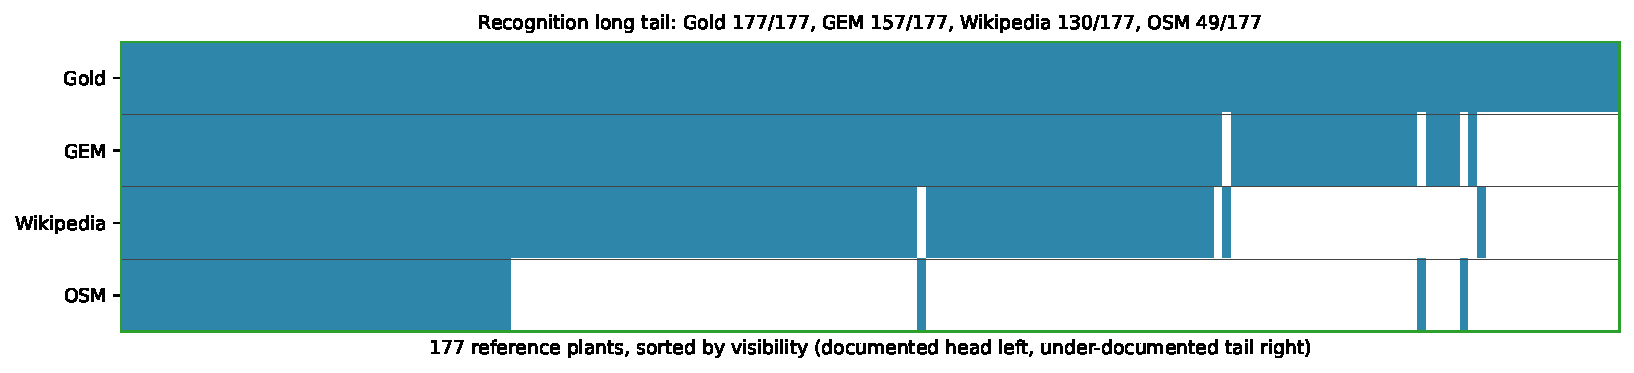
\includegraphics[width=\linewidth]{../../report/inputs/generated/fig_longtail_recognition.pdf}
\caption{The reference inventory covers plants that no other public
source holds. The \LongtailReference{} plants, sorted by descending visibility, are
checked against four recognition layers: the hand-compiled reference
itself (all \LongtailReference{}), the Global Energy Monitor tracker (\LongtailGem{}), Wikipedia
coverage (\LongtailWiki{}), and OpenStreetMap coverage (\LongtailOsm{} plants --- existing,
physically built infrastructure only). Well-documented operating plants
appear in every layer; the under-documented tail --- proposed and
planned projects from the PDP8 pipeline --- thins out layer by layer.
This tail is the reference's unique contribution, and the segment where
investing in a sourcing pipeline adds the most value. Counts re-derived
from
\texttt{data/reference/tab\_longtail\_layers.csv}.}\label{fig:longtail}
\end{figure}

\textbf{Statistical perimeters by use case.} What counts as a
``complete'' inventory is audience-relative, because each analytical use
draws a different lifecycle perimeter. Market dispatch and operational
modelling need only the \emph{operating} fleet. Investment analysis adds
the \emph{under-construction} and \emph{planned} tiers, read critically
for slippage risk. Development planning and energy-system modelling
extend the perimeter to \emph{proposed} projects, since the scenario
question is precisely which of them get built. Policy analysis and
energy-transition studies push furthest, retaining even \emph{cancelled}
and \emph{abandoned} projects, because the pattern of what was dropped
--- and why --- is itself the evidence. ``Complete'' therefore has no
audience-free definition. We take the researcher's perimeter, the
widest one: the reference aims to be exhaustive and detailed for the
whole economic and policy history of the thermal sector --- proposed,
cancelled, and abandoned projects included. The long tail is not noise
to prune; it is the research object. Built as this superset, the
reference lets each downstream use cut the narrower perimeter it
needs.

Neither the aggregators nor the community sources attempt what the task
demands: enumerate a national asset class in the open world, from facts
dispersed across heterogeneous documents partly in a non-Latin script,
and source every cell. Measuring how close AI systems come requires a
yardstick, which §\ref{sec:quality} defines.

\section{Quality dimensions for research-grade statistical datasets}\label{sec:quality}

Datasets can be assessed on four dimensions: accuracy, coherence,
provenance, and temporality. The decomposition compresses three
traditions: data-quality engineering
\citep{Wang-Richard1996:beyond-accuracy}, official-statistics governance
\citep{IMF2003:dqaf, UN2014:fundamental-principles}, and
philosophy-of-science empirical adequacy
\citep{vanFraassen1980:scientific-image}.

\begin{enumerate}
\def\labelenumi{\arabic{enumi}.}
\item
  \emph{Accuracy} asks whether the dataset contains the right assets and
  the right attributes. At the row level, this means recall (does the
  system find all relevant assets?) and precision (does it exclude
  non-assets and duplicates?). For a simple inventory table, this
  can be measured against a manually curated reference table using
  these two rates and their harmonic mean, the F1 score
  \citep{Hendrycks-Dan2021:mmlu, Wu-Xianjie2025:tablebench, Tenckhoff-Sonke2026:llmstructbench}.
  At the cell level, accuracy asks whether the attributes attached to
  each asset are correct: capacity, fuel type, location, operator,
  commissioning year, status, and so on. A system can therefore be good
  at finding the right assets but weak at describing them, or conversely
  reliable on attributes once the correct asset has been identified.
  Plausibility is not truth --- confidently-stated fabrications are the
  failure mode this dimension polices
  \citep{Lin-Stephanie2022:truthfulqa}.
\item
  \emph{Coherence} asks whether the dataset is internally and externally
  consistent. Internally, statistical tables carry control constraints:
  aggregate totals match subtotals, capacities are non-negative,
  duplicate units are counted once. Externally, the dataset must remain
  compatible with other available knowledge --- units, orders of
  magnitude, locations, technology types, and commissioning dates should
  all be plausible. A coherent dataset identifies conflicts between sources
  rather than silently overwriting them. A weak working test is whether
  repeated runs of the same system agree with one another
  \citep{Wang2022:self-consistency}; the stronger requirement is
  inferential closure --- the system derives and exposes all
  consequences of the available documents and accounting rules. This
  paper measures weak-internal coherence; the external axis is deferred
  to the Discussion.
\item
  \emph{Provenance} requires a pedigree for each data item: every row,
  and ideally every cell, traces back to specific passages, tables, or
  records in specific sources. Strong provenance means more than
  attaching a plausible citation --- the cited source must actually
  support the value claimed
  \citep{Gao-Tianyu2023:alce, Asai-Akari2024:self-rag, Es-Shahul2023:ragas}.
  We distinguish \emph{verifiable} provenance --- a citation is present
  and could in principle be checked --- from \emph{verified} provenance
  --- the citation was retrieved and confirmed to support the stated
  value. Verified provenance is the stronger standard; verifiable is the
  minimum floor. When sources contradict one another, the resolution ---
  which source was preferred and why --- is itself part of the
  provenance record.
\item
  \emph{Temporality} is not metadata added after the fact; it is part of
  the statistical fact itself. Energy infrastructure changes over time:
  projects are announced, financed, permitted, built, commissioned,
  repowered, mothballed, retired, cancelled, or renamed. Every value
  should therefore carry a best-effort ``as-of'' date or validity
  period, and notable status changes should be flagged. A statistical
  dataset should distinguish clearly current status from past reports,
  planned capacity from operating capacity, and source publication date
  from the date of the underlying fact. The currency / timeliness
  dimension is treated by Wang \& Strong
  \citeyearpar{Wang-Richard1996:beyond-accuracy} and by the IMF DQAF
  \citeyearpar{IMF2003:dqaf} but largely absent from LLM-evaluation
  practice, which the present work positions as a gap. This paper scopes
  to snapshot currency: the table describes the fleet at a reference
  date, each value carries a best-effort as-of date, and notable status
  changes are flagged. The fuller requirement --- supporting queries of
  the form ``what was the installed fleet in 2018?'' --- applies to
  scenario-projection use cases; it is addressed structurally in
  §\ref{sec:fusion} and discussed in \ref{sec:annex-temporality}.
\end{enumerate}

Of the four dimensions, accuracy is the only one whose measurement
requires a held-out gold reference. Coherence, provenance, and
temporality are reference-free: they can be assessed from the dataset
and its sources alone. The screening logic of this paper follows from
that asymmetry: where reference-free indicators correlate with accuracy,
they can estimate it --- screening out weak outputs without the
reference. The experiments exercise this logic directly
(§\ref{sec:exp1}).

The task is not simply to generate a plausible inventory-shaped answer.
The statistical object is a dated, sourced, internally reconciled set of
claims about energy-system assets and events. Accuracy determines
whether the claims are correct; coherence determines whether they can
coexist; provenance determines whether they are auditable; and
temporality determines what period of the world they describe.

\section{AI capability landscape: from chatbots to agentic systems}\label{sec:capability}

\begin{quote}
\textbf{Glossary.} \emph{Parametric memory} --- facts a language model
has internalised in its weights during training, recalled without
consulting any external document. \emph{RAG (retrieval-augmented
generation)} --- supplementing the model's parametric memory at
inference time with passages fetched from an external corpus, so answers
can be grounded and cited. \emph{Agent} --- a model wrapped in a runtime
that lets it take multi-step actions (search the web, call tools, run
code, dispatch sub-agents) rather than emit a single reply. \emph{Token}
--- the sub-word unit a model reads and generates; billing and length
limits are measured in tokens. \emph{Temperature} --- the
sampling-randomness knob; temperature 0 makes decoding
near-deterministic, isolating prompt-driven variation from sampling
noise. \emph{F1} --- the harmonic mean of precision and recall; here,
row-level F1 scores how well an extracted plant list matches the
reference inventory.
\end{quote}

Between 2022 and 2025, AI capability advanced as an industry-wide
\emph{envelope}: the set of capabilities commercially attainable at a
given date, across labs. The systems that define this envelope vary
along four axes: \emph{training objective} (from raw text completion
through instruction-following to extended reasoning), \emph{input and
output media} (text, vision, audio, video), \emph{tool access} (none,
web browser, code execution, computer control), and \emph{product
workflow} (simple chat, single-task agent, deep research, coding agent,
autonomous task runner). The first two are properties of the model; the
last two are properties of the software that wraps it.
Figure~\ref{fig:capability-timeline} shows one projection of this
coordinate system: when each of eight capability surfaces first shipped
in a consumer-facing product, the threshold at which a working analyst
can rely on it, months after API or privileged-partner availability.

The envelope grows by integration. The integrations themselves
(retrieval, web access, reasoning surfaces, code execution, tool use,
and recursion) live in the runtime that wraps the model. What the model
contributes is \emph{conditioning}: a lab's investment in training the
model to exploit retrieved documents, tool calls, long reasoning
chains, and delegated sub-tasks is what lets it use each surface when
the framework exposes it. Each marker in
Figure~\ref{fig:capability-timeline} is the date the framework ×
trained-model × product triple first appears in a publicly available
commercial product.

Each row of Figure~\ref{fig:capability-timeline} corresponds to one
integration:

\begin{itemize}
\item
  \emph{Retrieval-augmented generation}
  \citep{Lewis-Patrick2020:rag, Gao-Yunfan2024:rag-survey} answers the
  coverage limit.
\item
  \emph{Reasoning} --- step-by-step deliberation first elicited by
  prompting \citep{Wei-Jason2022:cot}, later built in as computation
  the model spends before answering --- narrows the coherence limit on
  long, multi-source synthesis.
\item
  Their combination is the deep-research surface
  \citep{Wei-Jason2025:browsecomp}.
\item
  \emph{Code execution} lets the model verify arithmetic and produce
  executable artefacts.
\item
  \emph{External tool use} --- a standardised tool-connection protocol
  \citep{Yao-Shunyu2023:react} --- generalises code execution to an
  extensible registry of external services, with benchmarks on coding
  \citep{Jimenez-Carlos2024:swe-bench}, OS control
  \citep{Xie-Tianbao2024:osworld}, and general-assistant tasks
  \citep{Mialon-Gregoire2024:gaia}.
\item
  \emph{Agency} is the closure of that surface, when the tool-use set
  includes the model itself.
\end{itemize}

Each integration targets one or more of the §\ref{sec:quality} quality
limits; none addresses all four. The detailed per-lab shipping
order --- feature parallelism, the deep-research dependency, and the
DeepSeek negative case --- is given in \ref{sec:annex-rollout}.

Below these integrations sits \emph{articulation} --- the craft of
casting the problem into a query the system can answer. The
articulation is double: the problem must be cast as the analyst's
question, and the question as the LLM prompt. The LLM must answer the
question asked and follow the prompt; but the question must also match
the problem, and either link can fail on its own. A failure of the
first link is the \emph{Type-III error} \citep{Mitroff1974}: solving
the wrong problem --- in LLM work, a well-executed answer to a
mis-posed question. Prompt engineering is the craft that addresses the
second link, from the analyst's question to the prompt the model
receives. Articulation also confounds every downstream quality metric:
a model that retrieves the correct fact but words it in a form the
extractor does not recognise produces a missing value indistinguishable
from a genuine coverage gap (developed in §\ref{sec:discussion}). The
experiments exercise articulation through structured prompts
(§\ref{sec:exp1} and §\ref{sec:exp2}); the verbatim prompts are
reproduced verbatim in \ref{sec:annex-exp1} and
\ref{sec:annex-exp2}.

\begin{figure}
\centering
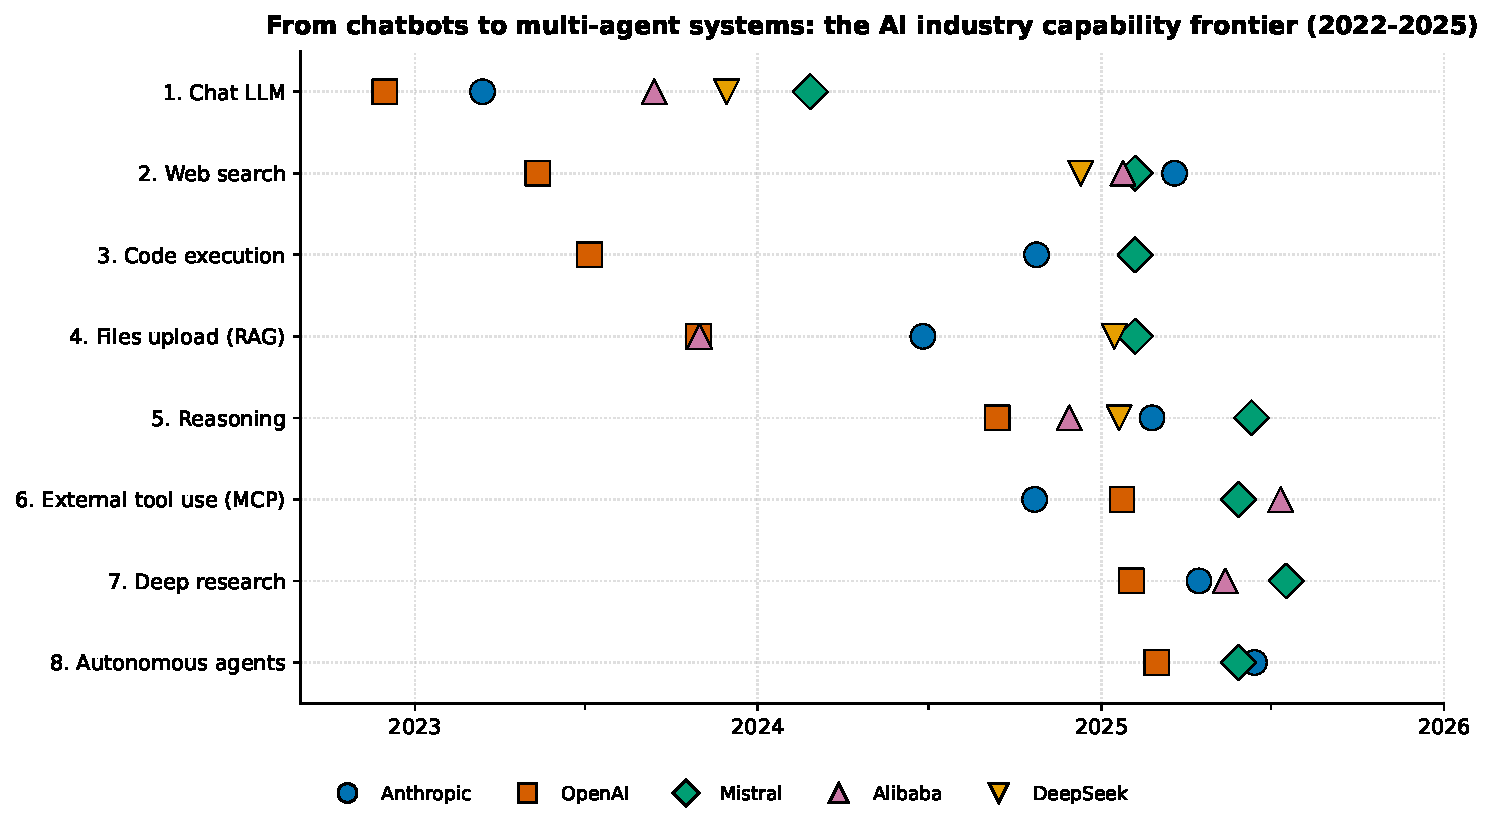
\includegraphics[width=\linewidth]{../../report/inputs/generated/fig_capability_timeline.pdf}
\caption{Empirical capability rollout across five leading AI labs. Each
capability is a feature of the lab's public commercial product, not a
property of the underlying model. Each row is a capability feature (1
chat LLM → 8 multi-agent recursion); each marker places when the named
lab first shipped that feature in a consumer-facing product. The figure
sets the experimental conditions: a lab's position on each row is the
capability set its system brings to §\ref{sec:exp1} and
§\ref{sec:exp2}. Source: author's compilation; per-lab primary
announcements documented in
\ref{sec:annex-rollout}.}\label{fig:capability-timeline}
\end{figure}

This capability envelope defines the conditions under which the
experiments run; whether any of it clears the §\ref{sec:quality} quality
bar is an empirical question. §\ref{sec:exp1} measures the parametric
floor --- what a bare model produces from memory --- and
§\ref{sec:exp2} tests the full agentic frontier.

\clearpage
\section{Experiment 1: parametric baseline}\label{sec:exp1}

Submitting a direct query to a large language model produces an
inventory-shaped answer, but not one that meets statistical or
scientific quality standards. Numbers shift between runs, citations are
absent or fabricated, and there is no way to tell which cells one should
trust.

\textbf{Cohorts.} The sweep dispatched 16 models (the
\texttt{modelset\_exp1\_journal} set in
\texttt{experiments/experiments.toml}). Two --- \texttt{qwen3.6-27b} and
\texttt{qwen3.6-plus} --- were dropped before analysis, leaving the
14-model analysis cohort (\texttt{modelset\_exp1\_batch2}) that backs
every per-model number, Figure~\ref{fig:direct-base},
Figure~\ref{fig:cost-quality}, and Figure~\ref{fig:reliability}. Every
figure caption below names the cohort it draws on.

\textbf{Experiment 1 --- Parametric baseline.} We query fourteen
language models from the \emph{modelset\_exp1\_batch2} set, spanning
three language families (EN/FR/ZH) and five laboratories from mid-range
through frontier-class systems, with a fixed inventory-specification
prompt (the full Doc-07 naive prompt,
\texttt{experiments/sota/protocol\_07\_naive\_prompt.md}, reproduced
verbatim in \ref{sec:annex-exp1}). No documents are
provided; models draw exclusively on parametric knowledge and receive a
system instruction forbidding web search. Each model is queried five
times at temperature zero, yielding \ExpOneNRuns{} runs against a \NumRefPlants-plant
reference inventory of Vietnamese thermal power plants (coal and gas,
all lifecycle statuses). Runs are evaluated by matching extracted plant
names against the reference using fuzzy string matching, yielding
row-level precision, recall, and F1; fuel type, operational status, and
province accuracy are scored at the cell level for matched rows. Cost in
USD and wall-clock time are recorded per run.

\textbf{A seeded recall bar: the answer key was already in the training
corpus.} These scores need an upper bound the reader can judge them
against. Before the experiment, the author's group published a
derivative of the reference --- the MOIT/PDP8 coal plant list --- on
Wikipedia; the experimental protocol therefore bans Wikipedia as a
\emph{justification} source (compliance audit in \ref{sec:annex-exp2}),
while permitting any source for \emph{lead generation}: a model may
legitimately recall a Wikipedia-seeded plant, it just may not cite
Wikipedia for it. The reference's content reached Wikipedia through a
deliberate group activity, not a benchmark instrument: an intern in the
author's group injected reference-derived content into the pre-existing
\emph{List of power stations in Vietnam} on 19 June 2019 (significantly
increasing its coverage; verifiable in the page history, revision
\texttt{902510278}), and \emph{List of coal power stations in Vietnam}
was split off on 5 July 2019 (provenance and diff in
\texttt{data/reference/PROVENANCE.md}). Both events predate the 2026-era
model cohort by roughly six and a half years --- comfortably before any
plausible training cutoff --- so the bar's validity is not in doubt for
the cohort; we report the comparison directionally because the project
does not record per-model cutoff dates. One caveat on coverage: the
built fleet (operating, retired) has been on these pages since mid-2019
and is firmly inside every cutoff, while much of the forward-looking
pipeline is PDP8-era (post-2019) content added after the June 2019
injection, so those rows may postdate some cutoffs. The recall bar is
therefore solidly substantiated for the built fleet and an upper-bound
heuristic for the pipeline tail. Wikipedia coverage of the reference is
thus the recall bar a competent parametric model ought to clear --- the
answer key was placed directly in the training corpus --- and grading
recall against it is not circular, because the bar measures retrieval,
not justification. The bar has two regimes (light-reviewed,
\ref{sec:annex-exp1}): the built fleet is covered at a 92\% mean
(operating 95\%, construction 80\%, permitted 100\%), while the
forward-looking pipeline sits at 55\% (proposed and announced; 73\%
aggregate). Scoring below the built-fleet bar is therefore not missing
obscure facts --- it is failing to retrieve knowledge demonstrably
present in the training corpus. The pipeline tail, which even Wikipedia
barely carries, is the reference's unique contribution; no parametric
source holds it.

\textbf{Results: model memory alone yields incomplete, unstable
inventories.} Across \ExpOneNRuns{} runs (\ExpOneNModels{} models × 5 repeats), all produced
usable tables, but row-level F1 ranges from \ExpOneFOneMin{} to \ExpOneFOneMax{}, with a mean of
\ExpOneFOneMean{}. Asking the same model the same question does not return the same
plants: DeepSeek V4-Flash ranges from F1 0.07 to 0.52 across 5 identical
runs --- a spread wider than the gap between many adjacent model means.
Even for correctly matched plants, attribute classification is uneven:
province accuracy is high (mean \ExpOneProvinceAcc{}) --- unsurprising, since Vietnamese
plants are typically named after the places that host them, so the name
itself usually gives away the province --- but fuel (\ExpOneFuelAcc{}) and status
(\ExpOneStatusAcc{}) remain mediocre, reflecting the finer coal-versus-gas and
lifecycle distinctions the models conflate. The status figure is partly
an artefact of vocabulary: ``Proposed'' --- the grouped status of
\textasciitilde\StatusProposedSharePct\% of the reference (\ref{sec:annex-recognition}) ---
has no equivalent in the prompt's controlled status vocabulary (the
cohort prompt's status definitions, aligned with Global Energy Monitor
vocabulary and reproduced in \ref{sec:annex-exp1}, offer
\texttt{Announced\ /\ Pre-permit\ /\ Permitted\ /\ Construction\ /\ Operating\ /\ Shelved\ /\ Cancelled\ /\ Retired}
--- no ``Proposed''), so a model that correctly recalls a proposed plant
has no admissible label to map it onto, which may mechanically depress
status accuracy. Consistent with that reading, excluding the proposed
stratum lifts mean status accuracy on the matched rows to
\ExpOneStatusAccExclProposed{}. Paying more does not reliably buy a better inventory:
Claude Opus 4.6 at \$1.23 total achieves mean F1 = 0.66, while
GPT-OSS-20B at \$0.01 reaches mean F1 = 0.02, but no monotonic
relationship between API cost and F1 holds across the lineup. The total
experiment cost is \$\CensusCostTotal{}.

An earlier sweep surfaced refusals rather than scores: in the archived
baseline sweep, GPT-5.5 declined the task on 3 of its 5 reps before the
\texttt{modelset\_exp1\_batch2} re-run reported above resolved
compliance. We retain the declined responses as data; the episode and
its reading against the §\ref{sec:quality} provenance bar are taken up
in the Discussion.

\begin{figure}
\centering
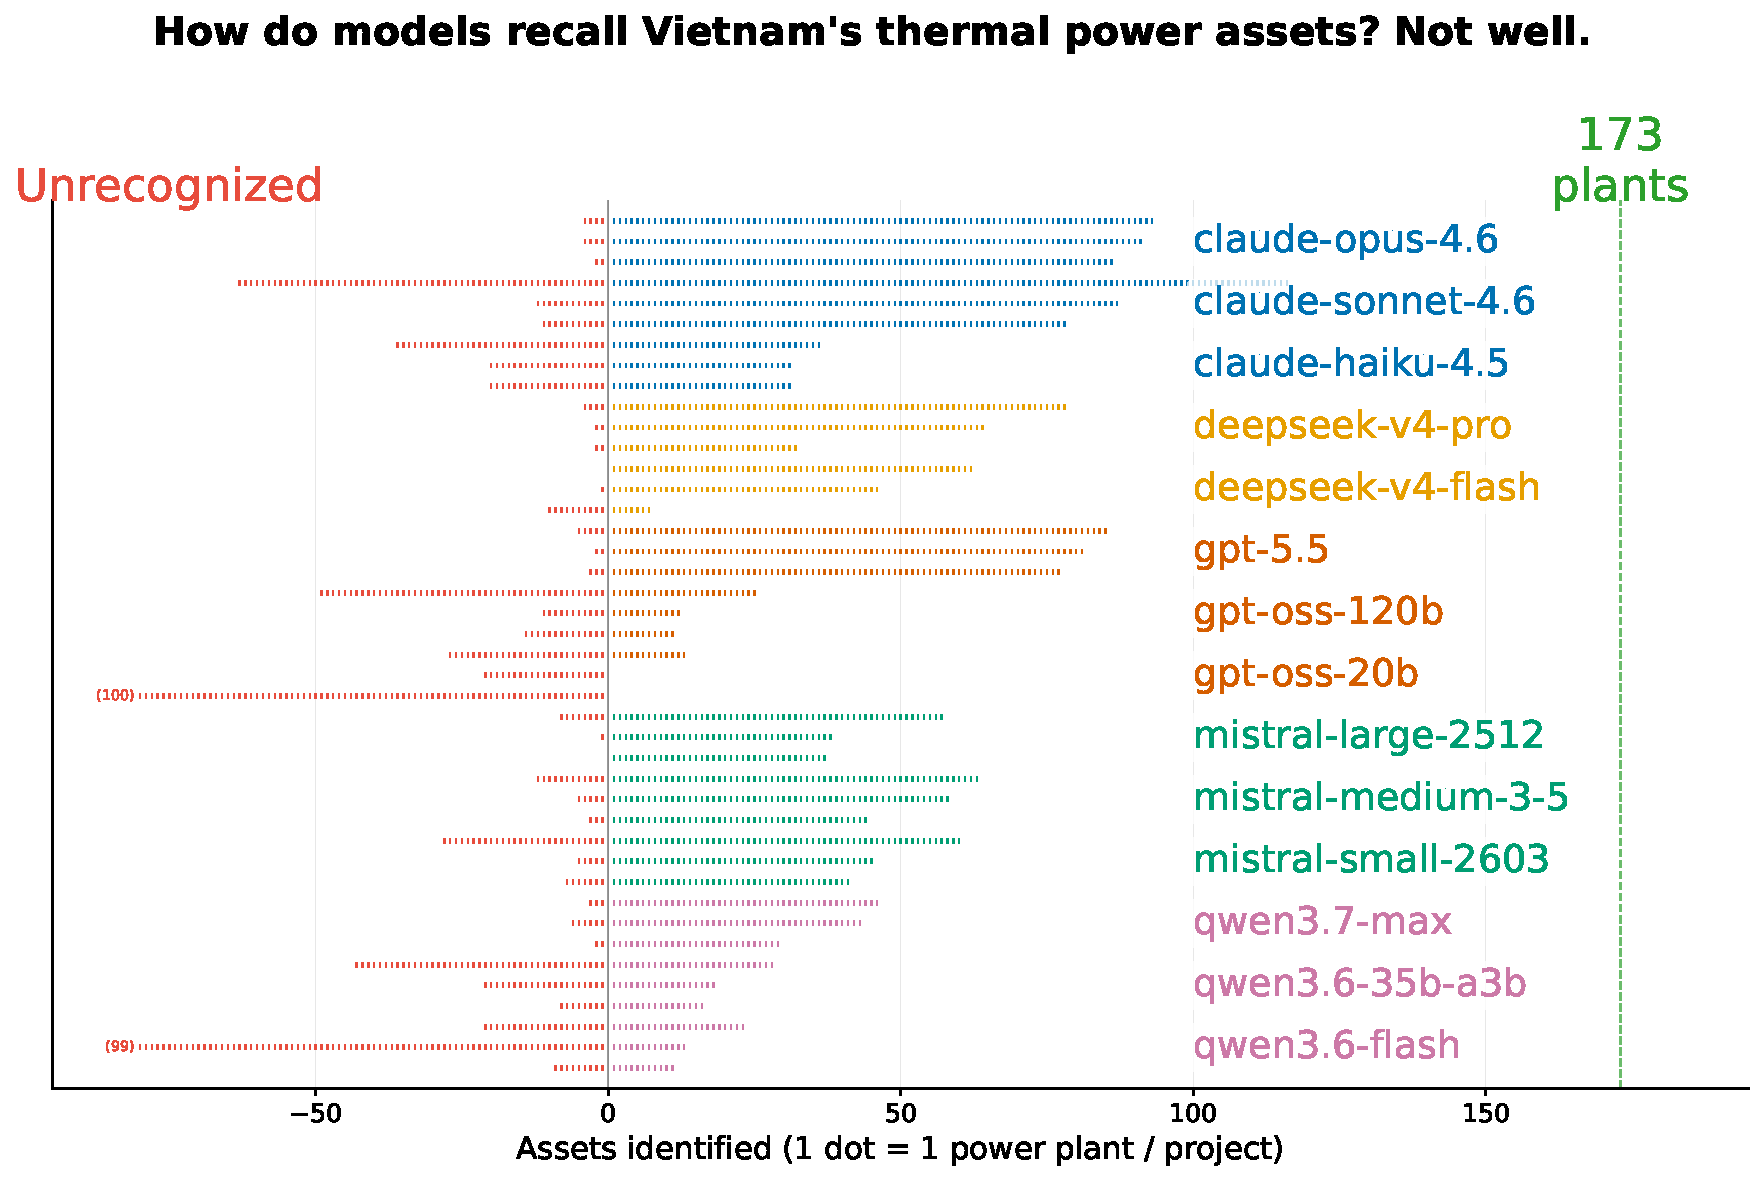
\includegraphics[width=\linewidth]{../../report/inputs/generated/fig_direct_p1_base.pdf}
\caption{No model approaches the full inventory from memory, and
repeated identical queries return different plants. Direct-query
performance across \NumCensusModels{} models and \CensusNumRuns{} runs on the \NumRefPlants-plant Vietnam
thermal reference: each bar is one run; family-coloured segments to the
right are correctly identified plants (TP), red segments to the left are
unmatched plants (FP: extracted but not in the reference). The dashed
green line marks the \NumRefPlants-plant reference; the light-grey dotted line
marks Wikipedia's light-reviewed coverage of all \NumRefPlants{} reference plants
(\WikiReviewedPct\%, \WikiReviewed/\NumRefPlants) ---
the seeded recall bar every model should clear, since that content sat
in the training corpus. Models grouped on the vertical
axis.}\label{fig:direct-base}
\end{figure}

\begin{figure}
\centering
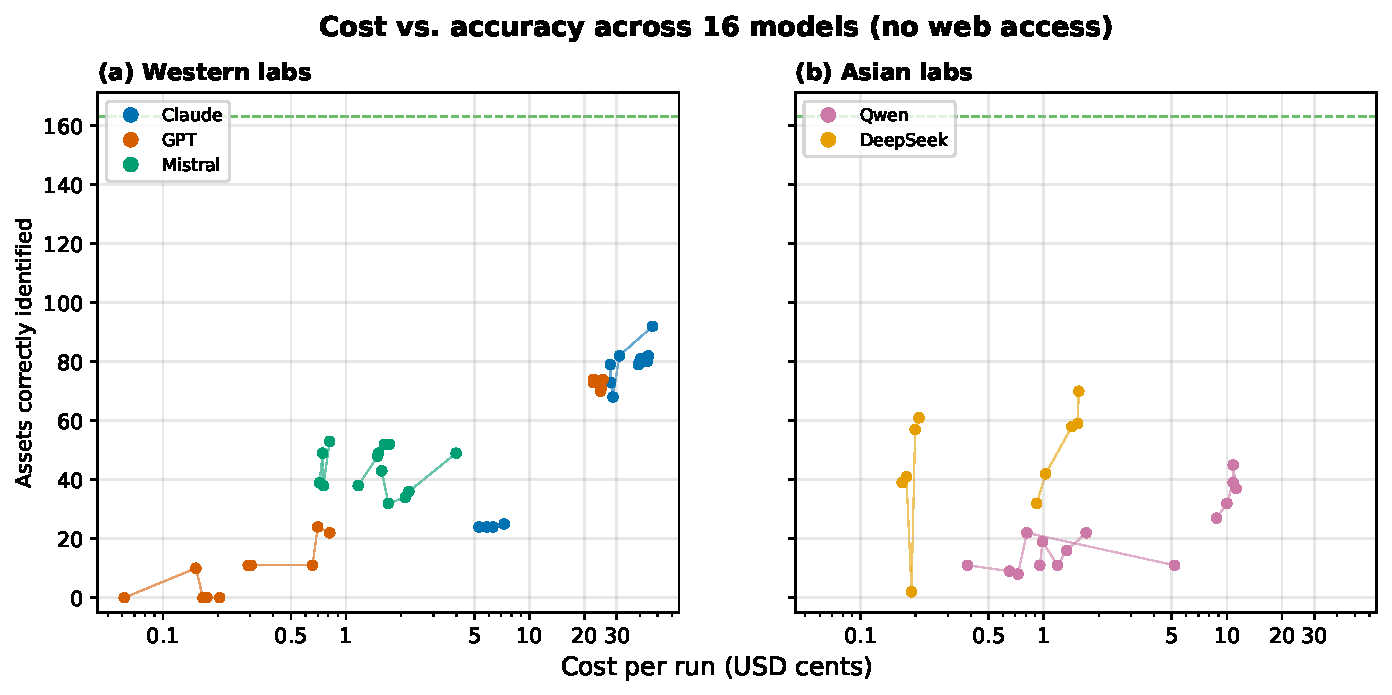
\includegraphics[width=\linewidth]{../../report/inputs/generated/fig_direct_cost_quality.pdf}
\caption{Paying more per call does not buy a proportionally better
inventory. Plants correctly identified vs cost per call across the
Experiment 1 lineup, split by architectural family across two panels
with shared axes: \textbf{panel (a)} Claude, GPT, Mistral; \textbf{panel
(b)} Qwen, DeepSeek. Each of the fourteen
\texttt{modelset\_exp1\_batch2} models contributes a filled square at
its pooled median true-positive count and a marker at every individual
rep, plotted at the rep's own per-call cost (cents USD, log scale); the
dashed line at \NumRefPlants{} marks the full Vietnam thermal inventory. Marker
shapes, colour palette, the per-rep cohort split, and the audit artifact
(\texttt{report/inputs/generated/cost\_quality.csv}) are detailed in
\ref{sec:annex-exp1}.}\label{fig:cost-quality}
\end{figure}

\textbf{A reference-free reliability grade separates the cohort.} The
§\ref{sec:quality} quality bar yields a model-level \emph{reliability}
grade that needs no reference data: call a run \emph{good} when it
scores zero on none of the twelve reference-free quality dimensions
(every dimension except the accuracy ones, which require the reference),
and grade each model by its count of good runs out of five.
Figure~\ref{fig:reliability} plots this grade against reference-based
accuracy. The cohort splits cleanly: nine models deliver four or five
good runs and F1 means of 0.41--0.67, while five models deliver at most
one good run (three of them none at all) and F1 means of 0.02--0.28 ---
the inaccurate models are also the unreliable ones (Spearman ρ = 0.78
between the two axes), so the label-free grade screens them out before
any reference is consulted. The disqualified set is essentially stable
under the gate's tuning choices --- indicator set and pass threshold ---
as the sensitivity sweep in \ref{sec:annex-exp1} shows; the
per-criterion breakdown behind the grade (which dimension each model
zeroes) is the quality-floor heatmap, also in \ref{sec:annex-exp1}.

\begin{figure}
\centering
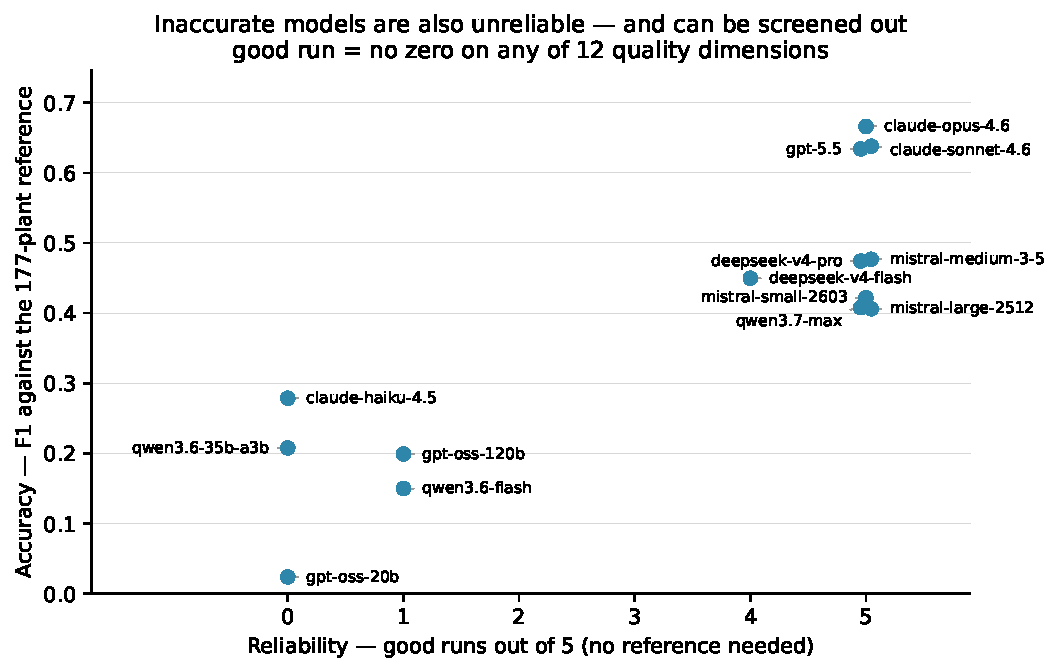
\includegraphics[width=\linewidth]{../../report/inputs/generated/fig_exp1_reliability.pdf}
\caption{Inaccurate models are also unreliable --- and a reference-free
screen can reject them. Model-level reliability vs accuracy for
Experiment 1 (14 models × 5 runs). X axis: reliability, the count of
good runs out of five, where a good run scores zero on none of the
twelve reference-free quality dimensions --- computable without any
reference data. Y axis: accuracy, the mean row-level F1 against the
\NumRefPlants-plant reference over the good runs; for the three models with zero
good runs (claude-haiku-4.5, gpt-oss-20b, qwen3.6-35b-a3b), no good run
exists, so the mean is taken over \textbf{all} five runs. Source
artifact: \texttt{experiments/derived/exp1\_cross\_eval.csv}; gate
sensitivity in \ref{sec:annex-exp1}.}\label{fig:reliability}
\end{figure}

\section{Experiment 2: frontier agents fall short on the measured quality dimensions}\label{sec:exp2}

How well do state-of-the-art tools perform at producing research-grade
statistical datasets? The parametric ceiling of §\ref{sec:exp1} is a
deliberately handicapped baseline --- no web, no tools, no reasoning
budget beyond what each model carries internally. The commercially
available frontier, by contrast, ships agents that combine extended
reasoning, web search, document ingestion, and tool use into a single
``deep research'' surface. The question is whether removing the
§\ref{sec:exp1} handicaps suffices to clear the §\ref{sec:quality}
quality bar. Even the best independent public tracker, Global Energy
Monitor, covers only \GemReviewedPct\% of the reference after light review
(\ref{sec:annex-exp1}); the frontier agents are therefore measured
against an inventory no single open database fully reproduces.

The quality dimensions §\ref{sec:exp2} measures are the
\emph{operational and accuracy} ones: row-level F1 against the
reference, coverage (plants enumerated), and per-row provenance counts
(Source 1 / Source 2 citation presence, \ref{sec:annex-suppfigs}). The
§\ref{sec:quality} dimensions that require \emph{peer cross-evaluation}
--- coherence, provenance support, and temporality scored on a rubric by
judging agents --- are deferred to Phase C (cross-model judging),
reserved for post-conference analysis; §\ref{sec:exp2}'s claims rest on
the F1, coverage, and citation-count metrics, not on the deferred
cross-eval scores.

\textbf{Experiment 2 --- frontier agents (\ref{sec:annex-exp2}).} We
conduct an experiment with four cloud AI agents at the May-2026
commercial frontier, each with extended reasoning and web access,
queried over direct vendor APIs (no browser automation): Anthropic
Claude Opus 4.6 (US, web\_search + adaptive thinking), OpenAI GPT-5.5
(US, Responses API + web\_search + reasoning), Mistral Large 2512 (FR,
Agents API + web\_search connector), and Qwen3-Max via DashScope (CN,
web\_search inside thinking mode). The fourth slot is
hypothesis-relevant rather than decorative: Chinese-language investor
and trade documents on Vietnamese power assets are under-indexed by
Western search. The experiment runs two arms over the same four agents
(N=5 each). \textbf{Arm 1 (naive)} --- a single-shot Doc-07 prompt,
web on; the null comparator. \textbf{Arm 2
(optimised, simple-harness multi-turn)} --- a multi-turn protocol in
which each agent first designs its own prompt and settings (Phase A),
runs once as a smoke gate (Phase B-0), then runs N=5 against a single
provider under a per-session cap of 50K tokens / \$3 (Phase B); this
constitutes a simple harness --- an LLM orchestrator (DeepSeek
classifier) controlling a loop with the tested LLM as the tool. The
naive-vs-optimised contrast isolates the protocol's contribution over
raw model capability. The naive arm is an independent sweep, not a
re-run of the §\ref{sec:exp1} parametric protocol, so its scores are not
directly comparable to §\ref{sec:exp1}'s per-model numbers;
within-Experiment-2 comparisons all use this common arm-1 sweep as their
baseline. Row-level F1 against the \NumRefPlants-plant reference is
now scored for all four arms (Table~\ref{tbl:exp2-2x2}); cross-model
judging on the four §\ref{sec:quality} dimensions remains reserved for
post-conference analysis (Phase C).

An anticipated objection: why not simply instruct the agents to merge
Wikipedia and the Global Energy Monitor tracker? Because the benchmark
evaluates a generic inventory method --- naming the best public sources
for this particular country and energy subsector would put the answer in
the question, and the resulting protocol would not transfer to a setting
where the strong sources are not known in advance. The agents get a fair
chance at discovering those sources themselves: the prompts reference
Global Energy Monitor only as a status-vocabulary standard, never as a
source to consult or merge; the public lists sit in
their training corpora (§\ref{sec:exp1}), web search is on, and the
optimised arm's multi-turn protocol explicitly encourages source
discovery. The one thing the protocol never discloses is where the
reference inventory itself is published.

\begin{table}[htbp]
\centering
\caption{\label{tbl:exp2-2x2}Experiment 2 --- row-level F1 and per-run
API cost (USD) by agent across the 2×2 factorial (query mode ×
documents), N=5 per cell. The §\ref{sec:exp2} narrative concerns the two
\textbf{registered} arms (naive vs optimised, documents = no). The two
documents = yes rows per agent are the \textbf{unregistered,
exploratory} conditions added during execution (\ref{sec:annex-exp2});
they are reported here for completeness, not as confirmatory tests.
Values generated from
\texttt{experiments/derived/tab\_exp2\_2x2.csv}'s pipeline.}
% Generated by aedist.tabulate_exp2_2x2 -- do not edit by hand.
\begin{tabular}{@{}lllll@{}}
\toprule
Agent & Query mode & Documents & F1 (mean) & Cost (mean, USD) \\
\midrule
Anthropic & naive (single-shot) & no & 0.60 & 2.02 \\
Anthropic & optimised (multi-turn) & no & 0.56 & 1.78 \\
Anthropic & naive (single-shot) & yes & 0.61 & 2.74 \\
Anthropic & optimised (multi-turn) & yes & 0.38 & 3.60 \\
Mistral & naive (single-shot) & no & 0.49 & 0.25 \\
Mistral & optimised (multi-turn) & no & 0.39 & 0.23 \\
Mistral & naive (single-shot) & yes & 0.59 & 0.06 \\
Mistral & optimised (multi-turn) & yes & 0.53 & 0.21 \\
OpenAI & naive (single-shot) & no & 0.63 & 0.27 \\
OpenAI & optimised (multi-turn) & no & 0.65 & 0.68 \\
OpenAI & naive (single-shot) & yes & 0.77 & 0.48 \\
OpenAI & optimised (multi-turn) & yes & 0.74 & 1.05 \\
Qwen & naive (single-shot) & no & 0.37 & 0.06 \\
Qwen & optimised (multi-turn) & no & 0.27 & 0.21 \\
Qwen & naive (single-shot) & yes & 0.62 & 0.30 \\
Qwen & optimised (multi-turn) & yes & 0.55 & 0.76 \\
\bottomrule
\end{tabular}

\end{table}

\begin{figure}
\centering
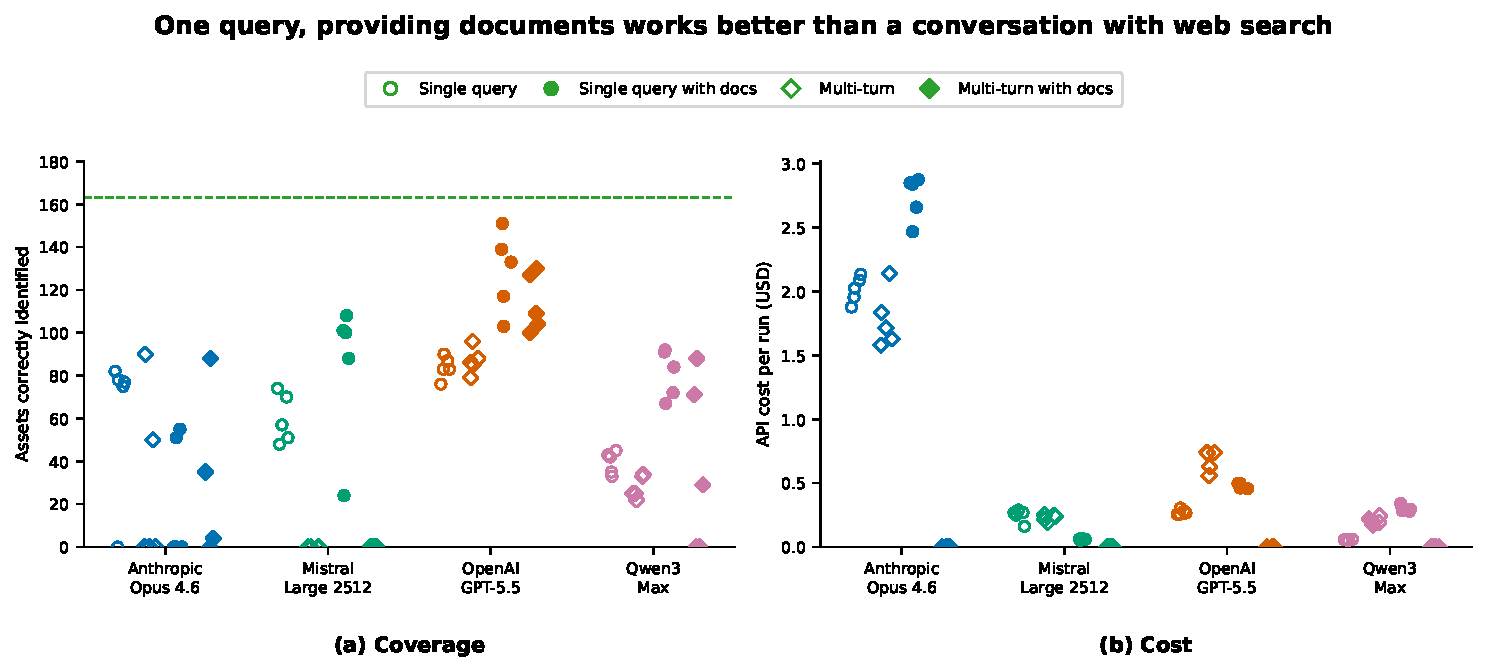
\includegraphics[width=\linewidth]{../../report/inputs/generated/fig_exp2_arms_comparison.pdf}
\caption{Web access lifts coverage, but no agent approaches the
reference --- and the multi-turn protocol costs 2--4× more for mixed
returns. Experiment 2 --- naive (arm 1, single-shot) vs optimised (arm
2, multi-turn) comparison, N=5 per agent. Panel (a): Plants found --- TP
bars (blue, upward, matched against the \NumRefPlants-plant reference) and FP bars
(red, downward, unmatched plants: extracted but not in the reference),
median over runs with scored outputs; left bar = arm 1, right bar = arm
2 per agent group. Grey bars indicate runs with no matched-row scores
available. Panel (b): API cost per run (USD), individual runs as scatter
points. Dashed green line marks the \NumRefPlants-plant reference count; the
light-grey dotted line marks GEM's light-reviewed coverage (\GemReviewedPct\%), the
best independent external database (\ref{sec:annex-exp1}). Row-level F1
against the \NumRefPlants-plant reference is now scored for all 80 runs; the 2×2
factorial analysis of F1 and cost (query mode × documents) is given in
Table~\ref{tbl:exp2-2x2} and detailed in \ref{sec:annex-exp2}. With N=4
agents as the blocking factor, effects are reported as directional
consistency (k/n agents agreeing in sign) rather than significance
tests, since the minimum attainable p at n=4 is 1/2⁴ =
0.0625.}\label{fig:exp2-arms}
\end{figure}

\textbf{Coverage: the best agent enumerates barely half the fleet.} For
agents in the naive arm (arm 1): Anthropic median 77 rows (4/5 usable,
one zero-row run); Mistral median 57 rows (range 48--74); OpenAI median
83 rows (range 76--90); Qwen median 42 rows (range 33--45) --- all
against the \NumRefPlants-plant reference. The optimised arm (arm 2) does not
change the picture: OpenAI median 86 rows versus arm 1 median 83 rows
(modest improvement; individual runs 79--96 vs 76--90); Qwen median 25
rows versus arm 1 median 42 rows (regression; Qwen's self-designed
protocol imposed a strict dual-source admissibility filter that
constrains coverage from Turn 1). The optimised protocol costs 2--4×
more per run than naive across all agents; OpenAI's ratio is most
extreme (median \$0.73 optimised vs \$0.27 naive). We did not find
published comparisons of frontier deep-research agents on
structured-output coverage at this granularity; the contrast is mixed
--- modest gain for OpenAI, regression for Qwen.

\textbf{Provenance: corroboration by a second source is the exception.}
Every Source 1, Source 2, and Notes cell across all 40 runs was parsed
to measure citation coverage and corroboration (see
\ref{sec:annex-suppfigs} for the full figure). OpenAI optimised is the
only agent to achieve both high coverage (79--96 rows) and near-complete
corroboration (77--88 rows with Source 2 --- approaching the full
diagonal). Qwen clusters near the diagonal at low coverage (22--45 rows
naive; 22--42 rows optimised), meaning nearly every plant it enumerates
carries a second source. Mistral naive produces near-zero corroboration
across all five runs (0 or 1 Source 2 citation per run) despite finding
48--74 rows. The most striking provenance gap is in the naive arm: all
five Mistral runs and several Anthropic runs return tables with Source 1
citations but no Source 2. We did not find published per-row provenance
analyses of this kind for frontier deep-research agents.

\textbf{Good documents equalise model performance.} The conditions in
which agents receive a curated document set are unregistered and
exploratory (\ref{sec:annex-exp2}), so the pattern is read tentatively
--- but it bears directly on where to invest. When agents receive the
same reference documents in a single query, the two weakest performers
climb toward the pack: Qwen lifts from F1 0.37 to 0.62 and Mistral from
0.49 to 0.59, against marginal movement for the already-strong Anthropic
(0.60 to 0.61). The spread across agents (max − min F1) narrows from
0.26 without documents to 0.18 with them --- three of the four now
converge near F1 0.61, with only OpenAI keeping headroom (0.77). This is
equalisation, not rescue: with a shared document set, which model runs
the query matters less than which documents it is handed. The effect is
specific to single-query prompting --- the multi-turn protocol with the
same documents does not equalise and in fact degrades Anthropic (0.61 to
0.38). Equalising at F1 ≈ 0.61 still leaves the cohort short of the
§\ref{sec:quality} quality bar; it suggests the binding constraint lies
in document quality rather than model capability, without resolving it. Extending
these observations to a wider model set (Sonnet, Mistral Medium/Small,
DeepSeek) is deferred --- no further API calls were made; the finding
rests entirely on the four-agent cohort already scored in
Table~\ref{tbl:exp2-2x2}.

\section{Need and potential for fusion}\label{sec:fusion}

The experiments in §\ref{sec:exp1} and §\ref{sec:exp2} establish that
the gap is real: recall from model memory is incomplete and volatile;
frontier agents with web access improve coverage but not provenance or
reproducibility. The Q\&A at the conference --- ``did you fuse the
results?'' --- points directly to the path forward. A naive union
already helps: pooling runs across models more than doubles recall
relative to the single-run mean (\AggUnionGainX×) at no new collection cost
(aggregation sweep in \ref{sec:annex-fusion}). Full treatment ---
estimating the unobserved share by linear programming against a control
total, applying capture--recapture estimation for the residual --- is
addressed in a companion paper in preparation (working title:
\emph{Capture--recapture estimation of under-documented infrastructure
inventories}).

The mirror-image lever buys precision: requiring at least two of the
four frontier models to agree nearly eliminates false positives --- F1
= \FusionRTwoEOneFFrac{} with \FusionRTwoEOneFP{} false positives on the Experiment 1 cohort, F1 = \FusionRTwoETwoOneDFFrac{}
with \FusionRTwoETwoOneDFP{} on the Experiment 2 naive arm (full results in
\ref{sec:annex-fusion}). Both levers reuse existing runs; the
structural answer to the single-model ceiling is a stateful pipeline
that invests in the corpus rather than the model --- a managed,
auditable knowledge base maintaining a sourced narrative inventory,
from which the statistical table derives as a dated snapshot. The
architecture rationale and the full factorial sweep are developed in
\ref{sec:annex-fusion}. To our knowledge, no published benchmark or
system targets open-world enumeration of a national asset class with
per-cell provenance at this granularity. Nor did we find a published
demonstration of the conjunction of per-cell provenance with per-cell
temporal validity in LLM-augmented inventories; demonstrating it is
part of the contribution we aim for in the follow-on paper.

\section{Discussion}\label{sec:discussion}

The two experiments and the fusion exercise support a consistent
reading. Memory alone is incomplete and volatile (§\ref{sec:exp1});
web access at the commercial frontier buys coverage but not provenance
or reproducibility, and a curated document set equalises the agents
(§\ref{sec:exp2}); pooling existing runs recovers coverage, and a
two-model agreement gate restores precision (§\ref{sec:fusion}). This
section examines what the measuring instrument can and cannot support
in that reading --- the F1 metric, its variance sources, and the
single-case design --- and closes with the research programme the
findings open.

\textbf{F1 is a useful but opaque aggregate.} Row-level F1 is the
primary metric in §\ref{sec:exp1} and §\ref{sec:exp2}: it is the
field's standard comparability unit for structured recall, and it is
computable without manual annotation. As an aggregate, it collapses
coverage (are the right assets present?),
freshness (are the values current?), articulation (was the query
well-specified?), and coherence (are the claims consistent?) into a
single score. A system can achieve high F1 by excelling on one
dimension while failing silently on others --- a well-articulated
prompt against a stale corpus, for example, can return complete,
internally consistent, but outdated values. The §\ref{sec:quality}
four-dimensional framework diagnoses \emph{where} a system fails once
F1 has ranked it. Readers should interpret F1 comparisons as aggregate
capability rankings, with the quality framework as the diagnostic
lens.

\textbf{F1 conflates facts never found with facts found but not
expressed.} Articulation --- the gap between analyst intent and model
query --- has a soft boundary with coverage. A model that retrieves the
correct fact but paraphrases it in a form the downstream extractor does
not recognise produces a missing value in the output table; the symptom
is indistinguishable from a genuine coverage gap. F1 therefore conflates
two distinct failure modes: facts the model never found, and facts the
model found but failed to express in extractable form. The structured
four-section prompt in §\ref{sec:exp1} is designed to close the
articulation gap; the residual F1 deficit is more likely to reflect true
coverage and freshness limits than articulation failures. But this
remains an assumption, not a measured separation. A third failure mode
belongs to the measuring instrument rather than the model: plant-name
matching is itself a named-entity recognition problem, and a true plant
reported under a name variant the LP matcher does not recognise is
scored as a false positive plus a false negative --- a matcher limit,
not a metric limit (\ref{sec:annex-exp1}).

\textbf{Interday drift is an unquantified variance source.} Beyond the
5-rep within-session spread, provider-side silent movement --- routing
changes, checkpoint updates --- shifts scores at fixed call shape and
seed: the top-up canary observed shifts up to \(\Delta\)F1 = 0.289 over
a 24-hour window (qwen3.6-27b, \ref{sec:annex-exp1}), an interday
variance the design observes but does not quantify.

\textbf{Refusal is evidence about the standard.} In the archived
baseline sweep (prompt \texttt{p1\_base}; runs preserved in
\texttt{experiments/archive/outputs/exp1/baseline/},
\ref{sec:annex-exp1}), GPT-5.5 declined the task on 3 of its 5
memory-only reps, opening with ``I can't honestly produce a complete,
primary-sourced inventory\ldots{}'' and refusing to fabricate URLs or
source citations from parametric knowledge alone; of the two completing
reps, one scored F1 = 0.64 and the other returned a single-row,
near-empty table (F1 = 0.00). The \texttt{modelset\_exp1\_batch2} re-run
reported in §\ref{sec:exp1} resolved compliance (all five reps
completed, F1 between 0.61 and 0.65), yet the declined responses are not
a missing data point to be imputed --- they are a signal about the bar
itself. The model judged that a complete, primary-sourced inventory
cannot honestly be produced from parametric memory and refused to
fabricate the citations the table format invites. Read against the
§\ref{sec:quality} provenance dimension, that refusal is the correct
response: the dimension polices confidently-stated fabrication, and a
system that declines rather than fabricates is clearing, not failing,
the auditability test the benchmark is built to measure. The other
models' fluent but unsourced tables are the contrasting failure mode.

\textbf{External coherence is harder to measure, for three compounding
reasons.} The §\ref{sec:quality} coherence criterion distinguishes
internal consistency (within the dataset) from external consistency
(against world knowledge). The experiments in this paper measure
internal coherence. First, the reference knowledge base is undefined:
checking whether a stated capacity is plausible requires specifying
which knowledge pool to check against (the RAG corpus, the model's
parametric memory, official statistics, or physical engineering
constraints), and these pools overlap imperfectly and carry different
reliability. Second, the checker's capability matters: a small model
used as evaluator has poor recall of world knowledge and will miss
genuine inconsistencies; a large frontier model has better recall but
may introduce its own confabulations as apparent corrections. Third, the
depth of reasoning required varies by claim: detecting that a 6000 MW
gas plant in a province with no pipeline access is incoherent requires
multi-step inference, not lookup. Phase C cross-evaluation (Exp 2)
partially engages external coherence, since the judging agents bring
parametric world knowledge, but does so implicitly and unsystematically.
A principled external-coherence metric remains future work.

\textbf{Internal coherence rejects the weakest runs without any
reference.} The reference list grades runs from the outside; an
exploratory analysis of the Experiment 1 outputs suggests the weakest
runs can be rejected without ground truth at all. Degenerate runs are
template-like: near-constant capacity and status columns (one run emits
496 rows, every one 1200 MW and ``Operating''). Within-run capacity
variability --- the number of distinct capacity values --- correlates
with reference-based F1 at Spearman ρ = 0.92 across the 70 runs. An
in-sample threshold rule rejects 23 of the 26 weakest runs with no false
rejection --- an existence proof rather than a validated detector, as
the cutoffs were tuned on the same 70 runs. Notably, the
internal-coherence indicators we already compute carry no such signal:
fabricated rows use impeccable controlled vocabulary and plausible
dates. This points to a two-level scoring design. The run-level screen
rates one output; above it, a model-level reliability grade aggregates
the screen across repetitions --- a model version whose five repetitions
all fail is disqualified as a source, independently of any single run.
In the vocabulary of intelligence evaluation (the NATO ``Admiralty''
grading of STANAG 2511), the run-level screen rates \emph{information
credibility} while the model-level grade rates \emph{source
reliability}. Making these scorers part of the standard pipeline is
future work. \ref{sec:annex-screen} tests whether the screen
discriminates good from bad runs of the \emph{same} model (removing the
across-model confound) and reports a model-stratified Kendall τ =
+\ScreenTauCap{} for cap\_distinct vs F1, positive in \ScreenPositiveSpearman/\ScreenNModels{} models.

\textbf{One case study, not a benchmark suite.} Every result above is
measured on a single case: the Vietnam thermal-plant fleet against one
\NumRefPlants-plant reference list. N = 1 at the dataset level means the findings
are existence proofs --- the task is hard, a curated corpus equalises
the agents, a reference-free screen and simple fusion rules work here
--- not generalisable benchmarks. The prompt templates, the LP matcher
parameters, and the quality bar were all developed against this
reference; transferring them to another country or asset class is a
replication study, not a configuration change. That is what makes the
next paragraph a research programme: each step is open to replication
and extension.

\textbf{From noisy runs to fused estimates.} The per-plant recognition
matrix in \ref{sec:annex-recognition} prefigures the research programme
this benchmark opens: each reference plant becomes a row observed by
many noisy runs --- precisely the input object of latent-truth discovery
and capture--recapture estimation. Within-model and across-model
coherence can be read directly from the row densities (famous plants
form dense rows, obscure ones sparse), and the operational core
separates visibly from the project-dominated tail. Fusing such
incomplete, differently-reliable lists into a single estimate --- and
bounding the residual share of plants that no source mentions by linear
programming against a control total, such as the regulator's installed
capacity per fuel \citep{HaDuong2005} --- is the axis of research these
row densities invite.

\section*{Related Work --- Methods}
\addcontentsline{toc}{section}{Related Work --- Methods}

\textbf{LLM parametric recall for structured extraction.} Petroni et al.
\citeyearpar{Petroni-Fabio2019:lm-as-kb} established that transformer
language models encode factual knowledge as implicit key-value
associations, enabling recall without retrieval. Roberts et al.
\citeyearpar{Roberts-Adam2020:closed-book-qa} extended this to
closed-book question answering, showing that large models recover
structured factual answers from parametric memory alone. More recent
work has measured the ceiling and limits of this capability: TruthfulQA
\citep{Lin-Stephanie2022:truthfulqa} quantifies the rate at which models
assert false claims confidently; MMLU \citep{Hendrycks-Dan2021:mmlu} and
TableBench \citep{Wu-Xianjie2025:tablebench} profile structured-task
accuracy across domains; LLM-StructBench
\citep{Tenckhoff-Sonke2026:llmstructbench} specifically probes
structured-output fidelity. Together these benchmarks confirm that
parametric recall is both real and unreliable: models plausibly populate
structured templates, but with no mechanism to distinguish remembered
facts from confident confabulation, and no provenance trail.

\textbf{Data quality frameworks.} The statistical quality standard the
paper applies derives from the information-quality literature. Wang and
Strong \citeyearpar{Wang-Richard1996:beyond-accuracy} decomposed
\emph{data quality} into four dimensions --- accuracy, completeness,
timeliness, and consistency --- and argued that ``accurate'' is
insufficient for practical information use. The IMF Data Quality
Assessment Framework \citep{IMF2003:dqaf} and the UN Fundamental
Principles of Official Statistics \citep{UN2014:fundamental-principles}
translate analogous criteria into governance norms for national accounts
and price statistics. Underpinning these practical frameworks is a
deeper epistemological requirement: van Fraassen's
\citeyearpar{vanFraassen1980:scientific-image} distinction between
empirical adequacy (model fits observations) and truth (model describes
unobserved reality). Applied to power-plant inventories, the distinction
sharpens: a table that ``looks right'' in aggregate may conceal
systematic coverage gaps for under-documented assets --- an inadequacy
invisible to F1 scores and visible only through provenance chains that
reach primary sources.

\textbf{RAG, grounding, and agentic architectures.} Retrieval-augmented
generation \citep{Lewis-Patrick2020:rag, Gao-Yunfan2024:rag-survey} is
the standard engineering response to the parametric-recall ceiling:
supplement model memory with retrieved passages, reducing confabulation
and enabling attribution. Grounding quality is then measurable: ALCE
\citep{Gao-Tianyu2023:alce} and RAGAS \citep{Es-Shahul2023:ragas}
evaluate whether each generated claim is traceable to a retrieved
passage, and Self-RAG \citep{Asai-Akari2024:self-rag} embeds retrieval
decisions as model outputs rather than preprocessing steps. At the
frontier, agent benchmarks --- GAIA \citep{Mialon-Gregoire2024:gaia} and
BrowseComp \citep{Wei-Jason2025:browsecomp} --- require multi-step tool
use and web navigation to answer questions that cannot be resolved from
parametric memory or a single retrieved passage. This ladder from
parametric recall through RAG to deep-research agents is the
architecture ladder the paper traverses.

\textbf{The gap this paper addresses.} The open-energy-database
literature provides the motivating need but not the construction method
for under-documented settings. The LLM-grounding literature provides
tools for source-attributed extraction but has not been applied to
systematic power-plant inventory construction. The data-quality
literature provides the evaluation criteria but no application to
LLM-generated tables. To our knowledge, no published work combines
agentic structured extraction with explicit per-row provenance against a
held-out reference inventory for a national power-plant dataset in an
under-documented jurisdiction --- the conjunction of pipeline,
provenance, reference evaluation, and data-quality framework that this
paper studies.

\section{Conclusion}\label{sec:conclusion}

As of mid-2026, AI systems queried with or without web access do not
reliably produce research-grade statistical inventories, and the
evidence points toward a conjecture about why: the binding constraint is
the data, not the model. Each claim in that sentence rests on a measured
result. That the task is hard is established twice. In the memory-only
baseline (§\ref{sec:exp1}), fourteen models score row-level F1 between
\ExpOneFOneMin{} and \ExpOneFOneMax{} with high within-model variance, below an available
ceiling: group-seeded Wikipedia lists alone cover 92\% of the built
fleet and sat in the training corpus for years, yet the models failed to
retrieve them. At the commercial frontier (§\ref{sec:exp2}), agents with
web access and extended reasoning enumerate at best around half the
fleet and fall short on the quality dimensions measured here (row-level
accuracy, coverage, and citation-based provenance), with the
rubric-scored dimensions (coherence, provenance support, temporality)
deferred to a planned cross-evaluation. The conjecture itself rests on
the exploratory, unregistered documents condition: handing the same
agents a curated document set in a single query equalises three of the
four, though the multi-turn protocol does not replicate the effect
(§\ref{sec:exp2}). Two levers already deliver without any new data
collection. The reference-free screen rejects the weakest outputs
without ground truth: within-run capacity variability tracks
reference-based F1 (Spearman ρ = 0.92, pooled across models and
in-sample; within-model signal positive but modest,
\ref{sec:annex-screen}). Fusion recovers coverage: pooling runs across
models finds plants no single model reliably finds, and requiring two
models to agree nearly eliminates false positives (§\ref{sec:fusion}).
If the constraint is indeed the documents, the path to research-grade
quality runs through the sourcing pipeline: assembling, curating, and
resolving documents in an auditable knowledge base from which
statistical tables derive as dated snapshots, with human-in-the-loop
resolution and multi-run fusion, not through a stronger model or a
single heroic prompt. For the many countries whose statistical systems
cannot yet supply machine-readable asset inventories, that is where the
investment should go.

\section*{Acknowledgements}
\addcontentsline{toc}{section}{Acknowledgements}

We thank Econom'IA 2026 participants for their comments, in particular
those that led to the updated reference list, the per-plant recognition
matrix, and the status-composition analysis of task difficulty in the
annex.

\textbf{Data \& Code Availability.} Code and data are available at
https://github.com/MinhHaDuong/aedist-technical-report (CC BY 4.0).

\textbf{Funding.} This work was supported by CNRS/CIRED.

\textbf{Author contributions and conflicts of interest.} The author
compiled the \NumRefPlants-plant reference list, and an intern in the author's
group, working under the author's supervision, seeded reference-derived
content into the relevant Wikipedia pages in June 2019; the author also
made minor edits to those pages directly (§\ref{sec:exp1}; provenance in
\texttt{data/reference/PROVENANCE.md}). Both the benchmark reference and
part of its Wikipedia coverage therefore originate from the author's
group; this dual role is disclosed, and the reference list is provided
as a supplementary artifact with per-plant source citations.

\renewcommand{\refname}{Bibliography}
\bibliography{../../report/refs}

\appendix
\renewcommand{\thesection}{Annex \Alph{section}}
\renewcommand{\thefigure}{S\arabic{figure}}
% Disambiguate hyperref anchors after the figure-counter reset, otherwise the
% S-series figures collide with body figures ("Object @figure.N already defined")
\renewcommand{\theHfigure}{S\arabic{figure}}
\setcounter{figure}{0}

\section{Temporality: state representations vs.~event representations}\label{sec:annex-temporality}

The temporality dimension in §\ref{sec:quality} measures \emph{snapshot
currency}: whether each value carries a best-effort ``as-of'' date and
whether notable status changes are flagged. This is a deliberately
scoped definition; a richer requirement exists and is worth naming
precisely.

The distinction at issue is between \emph{state} representations (a
snapshot describing the fleet as it stands at a reference date) and
\emph{event} representations (a log of the installation, retirement, and
reclassification events that change that state over time). Integrated
Assessment Models (REMIND, MESSAGE, TIMES/MARKAL, GCAM) reconcile the
two via \emph{capacity vintaging}: every installation event creates a
stock unit tagged with a birthdate and a lifetime, so system state at
time T is the integral of all past installation events minus
retirements. A database feeding such a model should, in principle,
support reconstruction of system state at \emph{any} reference date, not
only the most recent snapshot.

\textbf{Two distinct quality requirements.} This distinction yields two
separable temporality criteria for an energy-asset database:

\begin{itemize}
\tightlist
\item
  \textbf{T1 --- Snapshot currency}: each value carries a
  source-publication date and a best-effort ``as-of'' validity period;
  status changes since that date are flagged. This is what
  §\ref{sec:quality} requires and what the experiments measure.
\item
  \textbf{T2 --- Historical reconstructability}: the database supports
  queries of the form ``what was the installed fleet as of 2018?'' This
  requires logging the events (commissioning, retirement, capacity
  revision, status reclassification) that change state over time --- the
  approach taken by Global Energy Monitor rather than the Global
  Powerplant Database snapshot model.
\end{itemize}

The present paper scopes to T1. T2 is acknowledged as the stronger
requirement for IAM and scenario-projection use cases; it is not in
scope here. A GEM-style event log may become necessary when implementing
the verified-provenance layer (§\ref{sec:fusion}, future work) --- each
verification act is itself a timestamped event --- but that design
choice is deferred to a subsequent paper.

The narrative inventory component of §\ref{sec:fusion} handles
longitudinal aspects pragmatically: plant histories, PDP-cycle
reclassifications, and developer-name changes appear as free-text
annotations rather than as structured event records. This is a
deliberate scoping decision, not an architectural commitment.

\textbf{International energy statistics practice.} The T1/T2 distinction
maps directly onto the revision policies and data-quality frameworks
developed by the major international energy statistics bodies. The IEA
\emph{Energy Statistics Manual} \citep{IEA2004:energy-statistics-manual}
establishes the canonical treatment of reference-date conventions in
national energy balances: every supply and consumption entry carries a
``reference year'' and a ``publication year,'' and subsequent revisions
are tracked explicitly. The flow vs.~stock distinction in energy
accounts --- the tension between a snapshot of installed capacity and
the transaction log of commissionings and retirements --- is precisely
the state-vs-event distinction above, codified as professional practice.
The UN \emph{International Recommendations for Energy Statistics}
\citep{UNSD2012:ires} extends this to coverage and timeliness criteria,
noting that data quality includes not only accuracy but also currency: a
figure is not merely right or wrong, it has a validity window.
Eurostat's energy balance methodology
\citep{Eurostat2019:energy-balance-guide} adds the EU-specific
harmonisation layer: because member-state estimates are subsequently
revised when Eurostat reconciles supply-use tables, a snapshot of the
European fleet at any given date inherits a structured revision
calendar.

From these frameworks, the T1 requirement (snapshot currency with
source-publication date) corresponds to the notion of currency at
reference date: every record is tagged with the source-publication year
and flagged if the underlying situation may have changed since. The T2
requirement (historical reconstructability) corresponds to the practice
of maintaining a revision log: the ability to answer ``what did the
inventory show as of year Y?'' requires recording each revision event,
not only overwriting the current figure. The energy-statistics bodies
address both requirements; the databases evaluated in this paper satisfy
T1 in part and T2 not at all, which is consistent with the IAM gap
identified in §\ref{sec:exp2}.

\section{Experiment 1: Technical specification}\label{sec:annex-exp1}

\subsection*{Task}
\addcontentsline{toc}{subsection}{Task}

Identify all thermal power plants in Vietnam from parametric model
knowledge alone. The target population is defined by the reference
inventory
\texttt{data/reference/vietnam\_thermal\_plants\_v2\_classified.csv}:
\NumRefPlants{} plant-level records covering coal (\RefCoalCount) and gas/gas-oil (\RefGasOilCount), across
all lifecycle statuses (operational, under construction, proposed,
planned, cancelled, retired). The reference was compiled by the author
from primary sources (PDP7, PDP7A, PDP8 annexes, EVN annual reports,
MOIT decisions) and is version-locked for this experiment.

\subsection*{Reference dataset provenance}
\addcontentsline{toc}{subsection}{Reference dataset provenance}

The reference inventory was assembled by single-author manual
compilation, cross-referenced against the 18 source documents
snapshotted in \texttt{data/rag\_corpus/} (PDP7, PDP7A and PDP8 annex
tables, EVN annual reports, Report\_32, Report\_58, Study E542 unit
tables) plus a small number of MOIT decisions consulted off-corpus by
the author. The broader quality framework that motivates the design is
documented in \texttt{docs/quality-grounding.md}. The dataset is
version-locked (2026-05-20) for Experiments 1 and 2; per-row source
priority, the full file inventory, and MOIT decision identifiers are
recorded in \texttt{data/reference/PROVENANCE.md}.

Residual uncertainty concentrates in the 68 ``proposed'' and 21
``planned'' rows: these forward-looking statuses carry the highest
volatility across PDP cycles. The three cases most likely to shift
status, capacity, or developer between the freeze date and any
downstream use are LNG Cái Mép Hạ (Bà Rịa-Vũng Tàu, 6000 MWe), LNG Hà
Tĩnh (6000 MWe), and Dung Quat SEZ J-Power Phase I (Quảng Ngãi, 2400 MWe
coal). To our knowledge, no independent per-plant audit-trail dataset
exists for Vietnam's thermal fleet, and we did not find a second
human-curated reference at comparable granularity; the closest available
external check is Global Energy Monitor (GEM, \GemDistinct{} distinct plants;
snapshot exported no later than 2026-04-02, the date it entered version
control), against which we report a light-reviewed concordance in
Table~\ref{tbl:source-concordance}.

\textbf{Source concordance (reference vs GEM and Wikipedia).} GEM covers
\GemReviewed{} of the \NumRefPlants{} reference plants (\GemReviewedPct\%) after light review --- more
matches than GEM's \GemDistinct{} distinct plants because matching operates at the
reference's phase grain: one GEM plant row can match several reference
phase rows (e.g.~successive phases of the same site ---
\texttt{gem\_thermal.csv} has 153 rows under \GemDistinct{} distinct plant names).
Wikipedia (coal list + general-page gas section) covers \WikiReviewed{} (\WikiReviewedPct\%).
Neither is a superset: GEM retains 12 cancelled or announced plants the
reference excludes, while the reference adds the PDP8 LNG pipeline GEM
lacks (the 20 reference-only rows, concentrated in ``proposed''). The
built fleet is well covered by both; the divergence is in the
forward-looking tail, exactly where the reference's contribution lies.

\begin{table}
\centering
\caption{\label{tbl:source-concordance}Source concordance by status,
generated from \texttt{data/reference/tab\_source\_concordance.csv}.
Coverage is \textbf{light-reviewed} --- an ASCII-fold pass recovers
Vietnamese-diacritic naming variants the LP matcher floors (``Cà Mau I''
vs ``Ca Mau 1''), which slightly over-counts via phase/grain mismatch
(one source row ↔ several reference phases), so the percentages are
upper bounds --- quantified on the reference itself:
\texttt{partial\_ratio} ≥ 90 exposes \PhaseCollisionPairsNinety{}
distinct-plant name pairs, the unit-number veto leaves
\PhaseCollisionResidualNinety{} of them matchable, and the scored runs
realise \RealisedFuzzyBelowNinety{} fuzzy matches below the threshold.
Full per-plant human
reconciliation is deferred (post-arXiv).}
% Auto-generated by aedist.tabulate_source_concordance — do not edit.
\begin{tabular}{@{}lrrrr@{}}
\toprule
Status & Reference & GEM matched & GEM-only & Wikipedia matched \\
\midrule
Proposed & 68 & 53 & 2 & 37 \\
Planned & 21 & 21 & 0 & 18 \\
Under construction & 10 & 10 & 0 & 8 \\
Operational & 56 & 52 & 0 & 53 \\
Retired & 2 & 2 & 0 & 2 \\
Cancelled & 20 & 19 & 10 & 12 \\
\midrule
\textbf{All} & \textbf{177} & \textbf{157} & \textbf{12} & \textbf{130} \\
\bottomrule
\end{tabular}

\end{table}

\subsection*{Prompts}
\addcontentsline{toc}{subsection}{Prompts}

\textbf{Archived baseline prompt (2026-05-20 cohort).} The archived
baseline sweep --- the earlier cohort in which the GPT-5.5 refusals
occurred --- used the locked composition of two modules from
\texttt{experiments/prompts/modules/}: \texttt{2\_goal.txt} (task
declaration) and \texttt{5\_table.txt} (structured table specification).
These are the implicit ``always'' pair --- every sweep includes them;
ablations opt in to additional modules. The assembled prompt is the
concatenation in filename lex order, joined by a blank line:

\begin{quote}
\textbf{\#\# Goal}

Produce a complete, primary-sourced reference inventory of Vietnam's
past, present and future thermal generation assets (>
30MWe) structured as follows:

\textbf{\#\# Structured power plants table}

Tabulate for every thermal power plant in Vietnam:

Name (Vietnamese) | Name (English) | Province
| Fuel | Technology | Units × MW |
Total MWe | Status | COD | Owner/Developer
| Source 1 | Source 2 | Notes |

Where: - Fuel: Coal / Domestic gas / Imported LNG - Technology (coal):
Subcritical / Supercritical / USC - Technology (gas): CCGT / OCGT -
Status: Approved / Planned / Operational / Under construction /
Suspended / Cancelled / Retired - Total MWe: Include units >
30MWe. - COD: Actual or expected commercial operation date - Sources:
specify where in the document, include URL

Output format: Markdown.
\end{quote}

No persona, no narratives, no quality bullets --- those land in ablation
sweeps, not the archived baseline. The status enumeration above is the
as-sent text from the archived records; the \texttt{5\_table.txt} module
file was aligned to the Global Energy Monitor status vocabulary only
after this cohort ran, which the analysis-cohort prompt below reflects.

\textbf{Analysis-cohort prompt (Doc-07).} The fourteen-model analysis
cohort (\texttt{modelset\_exp1\_batch2}, the cohort behind every
per-model number in §\ref{sec:exp1}) received the full Doc-07 naive
prompt --- \texttt{experiments/sota/protocol\_07\_naive\_prompt.md} ---
verbatim as the sole user message (trailing newline stripped by the
worker), at temperature 0, seed 42, \texttt{max\_tokens} 65536, web
access off; this was verified against the archived per-run records. The
prompt in full:

\begin{quote}\small
\textbf{\# GOAL}

Produce a complete, primary-sourced reference inventory of Vietnam's
past, present and future thermal generation assets (> 30 MWe). Begin the
document directly with the inventory table — no title, no preamble, no
overview section. Structure it as follows:

\begin{itemize}
\tightlist
\item
  the plant inventory: \textbf{exactly one pipe table}, never split into
  sub-tables by status, fuel, province, or any other dimension. Columns
  in this exact order: Name (Vietnamese), Name (English), Province, Fuel
  (Coal / Domestic gas / Imported LNG), Technology (Subcritical /
  Supercritical / USC for coal; CCGT / OCGT for gas), Units × MW, Total
  MWe, Status, Status as-of-date, COD, Owner/Developer, Confidence,
  Source 1, Source 2, Notes. Do not add statistical summary,
  cross-tabulation, or any other pipe tables; fold aggregate statistics
  into prose.
\item
  per-asset or per-project explanatory notes: for each asset that
  warrants it (major, disputed, ambiguous, or historically important), a
  concise sourced note covering development history, notable issues, and
  confidence-qualified attributes. Straightforward operational assets
  need no note.
\item
  an annotated bibliography of every source cited (full citation; URL
  when available; original-language title plus English translation for
  non-English sources; summary annotation of what was drawn from each)
\end{itemize}

Scope includes all thermal assets > 30 MWe at any stage of the
lifecycle, including shelved or cancelled projects.

When uncertain, mark confidence LOW and explain why in the Notes field.
Never fabricate sources or URLs; write ``URL not verified'' if you
cannot locate the exact handle. Include known plants even without a
primary source rather than omitting them.

Output format: Markdown.

\textbf{\# QUALITY DIMENSIONS}

Your output is judged on four axes:

\begin{enumerate}
\tightlist
\item
  \emph{Accuracy} — right assets and right attributes. Row level: recall
  and precision against a curated reference (F1). Cell level: capacity,
  fuel, location, operator, COD, status correct. Confident fabrication
  is the policed failure mode.
\item
  \emph{Coherence} — internally and externally consistent. Totals
  reconcile with known subtotals; no negative capacities, no
  double-counted units, no cross-row contradiction; values plausible in
  unit, magnitude, geography, technology, date. Conflicting sources
  reconciled explicitly (which chosen and why), not silently.
\item
  \emph{Provenance} — each value traces to a source that actually
  supports it, not a merely plausible citation. Two independent
  primaries is the ideal; one primary, a regulator database, or a marked
  secondary is weaker but acceptable if its status is explicit.
  Unsupported values are the failure.
\item
  \emph{Temporality} — every value carries a best-effort as-of date;
  status changes are flagged. Distinguish current status from past
  reports, planned from operating capacity, source date from fact date.
\end{enumerate}

We prefer a comprehensive inventory with uncertainty clearly expressed
over a shortlist of well-known assets.

\textbf{\# CONTEXT}

\textbf{\#\# Source quality management}

Two distinct epistemic roles — do not conflate them:

\begin{itemize}
\tightlist
\item
  Discovery \& characterization: parametric knowledge and web search,
  including tertiary sources, MAY be used to generate leads, locate
  assets, and form initial hypotheses about attributes.
\item
  Justification in the final inventory: a claim can be justified ONLY by
  an admissible independently consulted source that actually supports
  it.
\end{itemize}

Admissible primary sources: official government documents;
regulator-aggregated official data; operator filings/press releases.

Admissible secondary sources: international-institution reports; bylined
trade press; industry trackers and data brokers that expose the primary
they cite.

Not admissible sources:

\begin{itemize}
\tightlist
\item
  Tertiary compilations (encyclopedias, Wikipedia/Wikidata/DBpedia,
  mirrors, aggregators re-syndicating without independent verification).
\item
  Any deposited dataset that does NOT expose, per value, the primary
  source it draws from — a DOI or repository deposit does not by itself
  confer admissibility.
\end{itemize}

Local-language sources are preferred but not required; when used,
include the original-language title plus an English translation in
brackets.

If a lead surfaces only via an inadmissible source, trace to its
original source and cite that; if none is found, record Source = ``not
found'', confidence LOW. In the table mention the inadmissible source in
Notes, not in Sources.

\textbf{\#\# Calibrated confidence vocabulary}

Each row in the inventory table carries a confidence level based on
evidence and agreement:

\begin{itemize}
\tightlist
\item
  HIGH = >=2 INDEPENDENT concordant sources, at least one is primary
\item
  MEDIUM = 1 primary source, OR a sourced aggregator citing a verifiable
  primary
\item
  LOW = secondary only / inferred / unresolved conflict / not found
\end{itemize}

Independence check (run BEFORE judging agreement):

\begin{itemize}
\tightlist
\item
  Trace each source to its origin; merge sources sharing one origin into
  ONE.
\item
  Sources re-syndicating Wikipedia/Wikidata are NOT independent and NOT
  admissible.
\item
  Filling both Source columns does not by itself confer HIGH;
  independence is required
\end{itemize}

Hard ceilings (override the above):

\begin{itemize}
\tightlist
\item
  Commercial operator self-reported not confirmed by an official source:
  cap claim at MEDIUM.
\item
  Status attested only by a source older than 24 months and unconfirmed
  since: cap status at MEDIUM (LOW if older than 48 months). Freshness
  is measured on the publication date of the most recent admissible
  source attesting the status — NOT on the older Status as-of-date.
\item
  ``Source = not found'' rows: LOW by construction.
\end{itemize}

Explanatory notes must state the confidence level for the row-level
existence/status claim and may additionally qualify one or two disputed
attributes (capacity, status, fuel, COD, owner/operator, or location).
Per qualified claim, state: value, confidence level, evidence type
(primary/secondary), and sources. When sources disagree, investigate for
transcription errors, time-based changes, and unit/translation issues;
follow the higher-tier source if unresolved, and add a note in the Notes
cell.

\textbf{\#\# Asset-row and status rules}

Each row corresponds to one asset record. The DEFAULT unit is the plant
/ unit-group, not the power center: when a site co-locates several
plants with distinct capacity, COD, owner/developer, fuel, status, or
financing (BOT/IPP) arrangements, each one is its own row. Aggregate to
center-level in a single row ONLY when detailed evidence is unavailable;
in that case mark the row ambiguous and explain the aggregation in
Notes. Conversely, do not split a single plant into multiple rows when
the only difference is individual generating units sharing one
commissioning, owner, and status — record these as Units × MW on one
row.

Status definitions (use these exact terms, aligned with Global Energy
Monitor vocabulary):

\begin{itemize}
\tightlist
\item
  Announced: described in government plans or corporate filings; no
  permits sought, no land acquired.
\item
  Pre-permit: environmental and regulatory approvals being sought; no
  permits issued yet.
\item
  Permitted: all required government approvals received; construction
  not yet started.
\item
  Construction: site preparation or EPC execution underway.
\item
  Operating: formally commissioned.
\item
  Shelved: previously active or advancing but progress halted without
  formal cancellation.
\item
  Cancelled: formally cancelled or replaced by another project.
\item
  Retired: permanently closed or decommissioned.
\end{itemize}

Capacity rule: Record nameplate electrical capacity in MWe when
available. If sources do not distinguish gross vs net, record the stated
MW value and note ``gross/net unspecified''. Do not mix thermal MW,
boiler capacity, steam output, or investment package capacity with
electrical MWe. For Units × MW, make arithmetic consistent with Total
MWe or explain discrepancies in Notes.

Explanatory notes discipline: The table comes first. Per-asset notes
follow the table and are selective: write one only for assets that are
major, disputed, ambiguous, or historically important. For
straightforward operational assets a compact Notes cell in the table is
sufficient; do not repeat it as a separate note.
\end{quote}

Two prompt-design limitations are acknowledged. First, although the
prompt asks the model to ``begin the document directly with the
inventory table'', it lacks a forced-prefix instruction (e.g.~start your
answer with \texttt{|\ Name}) that would constrain the first generated
tokens and simplify downstream parsing. Second, its status vocabulary
follows Global Energy Monitor and offers no label for the reference's
``Proposed'' stratum (\textasciitilde\StatusProposedSharePct\% of rows) nor for ``Planned''
--- mechanically depressing measured status accuracy, as discussed in
§\ref{sec:exp1}. Both are grounds for a revised-prompt rerun in the
journal version.

In both cohorts, every API call carried the same system instruction
explicitly forbidding web search (the two sweep configurations declare
the identical string): \emph{``You have no web search capability. Do not
claim to perform searches, do not invoke tools, do not fabricate URLs.
Answer from parametric knowledge only.''}

\subsection*{Models}
\addcontentsline{toc}{subsection}{Models}

Sixteen models from \texttt{modelset\_exp1\_journal} (v2, defined in
\texttt{experiments/experiments.toml}), organised around three language
families with multiple labs per family:

\begin{longtable}[]{@{}lllll@{}}
\toprule\noalign{}
Model & Lab & Family & Size class & Reasoning tokens* \\
\midrule\noalign{}
\endhead
\bottomrule\noalign{}
\endlastfoot
claude-opus-4.6 & Anthropic & EN & frontier & 0 \\
claude-sonnet-4.6 & Anthropic & EN & frontier & 0 \\
claude-haiku-4.5 & Anthropic & EN & mid & 0 \\
gpt-5.5 & OpenAI & EN & frontier & 1,537 \\
gpt-oss-120b & OpenAI & EN & large & 35 \\
gpt-oss-20b & OpenAI & EN & mid & 18 \\
mistral-small-2603 & Mistral & FR & mid & 0 \\
mistral-medium-3-5 & Mistral & FR & mid & 0 \\
mistral-large-2512 & Mistral & FR & frontier & 0 \\
qwen3.6-27b & Alibaba & ZH & mid & 5,735 \\
qwen3.6-35b-a3b & Alibaba & ZH & mid & 8,143 \\
qwen3.6-flash & Alibaba & ZH & mid & 7,971 \\
qwen3.6-plus & Alibaba & ZH & frontier & 6,677 \\
qwen3-max-thinking & Alibaba & ZH & frontier & 0 \\
deepseek-v4-pro & DeepSeek & ZH & frontier & 16,774 \\
deepseek-v4-flash & DeepSeek & ZH & mid & 775 \\
\end{longtable}

* Median over 3 runs.

Mistral's per-tier branding (Small 4 / Medium 3.5 / Large 3) is the
lab's own scheme and does not denote a generation order; we adopt their
naming verbatim. All sixteen models received identical call parameters
(T=0, seed=42, max\_tokens=32768, no-web system instruction). The only
reasoning-related signal sent was
\texttt{reasoning\_effort\ =\ "minimal"} for the two \texttt{gpt-oss-*}
entries, declared in the registry. The ``Reasoning tokens'' column
reports the median
\texttt{completion\_tokens\_details.reasoning\_tokens} field over the
post-fix top-up cohort (2026-05-21, \(N{\leq}3\) per model). The
original baseline cohort (2026-05-20) ran on a harness that stripped
\texttt{usage.completion\_tokens\_details} before writing records to
disk; the top-up sweep was issued post-fix with identical call shape to
recover the column. Two regimes are visible: Anthropic and Mistral
models report 0 reasoning tokens across all reps; DeepSeek V4, all
Qwen3.6 entries that we could run, GPT-OSS, and GPT-5.5 allocate between
dozens and 16,774 tokens to internal reasoning.
\texttt{qwen3-max-thinking} reports 0 despite the explicit naming:
OpenRouter does not expose reasoning tokens for this model in the
absence of an explicit \texttt{reasoning\_effort} flag.
\texttt{qwen3.6-flash} retains \(N{=}1\) post-fix because Alibaba's
free-tier upstream rate-limited additional attempts. For
\texttt{qwen3-max-thinking}, an early minimal-effort smoke produced 5/5
refusals; the no-effort lineup recovered 5/5 usable rows after a parser
fix that handles markdown section dividers inside structured-output
tables. The four Experiment 2 labs (Anthropic, OpenAI, Mistral, Alibaba)
each contribute their journal-pinned flagship --- Opus 4.6, GPT-5.5,
Mistral Large 2512, Qwen 3 Max Thinking --- so Experiment 2's ``deep
research vs parametric'' claim can be tested within-model (qwen3-max via
OpenRouter here, qwen3-max-2026-01-23 via DashScope in Experiment 2).
Opus 4.6 is preferred over the newer 4.7 for the parametric baseline
because 4.7's verbosity exceeds the \texttt{max\_tokens} budget on the
full Vietnam plant table. \textbf{GPT-5.5 declined this task on 3 of 5
reps in this archived baseline sweep (prompt \texttt{p1\_base})},
opening with ``I can't honestly produce a complete, primary-sourced
inventory\ldots{}'' and refusing to fabricate URLs or source citations
from parametric knowledge alone; the \texttt{modelset\_exp1\_batch2}
re-run reported in the body resolved compliance. We retained the
declined responses as data --- a model viewpoint on the request's
epistemic standard, not extraction noise.

\subsection*{Run parameters}
\addcontentsline{toc}{subsection}{Run parameters}

\begin{longtable}[]{@{}
  >{\raggedright\arraybackslash}p{(\linewidth - 4\tabcolsep) * \real{0.3333}}
  >{\raggedright\arraybackslash}p{(\linewidth - 4\tabcolsep) * \real{0.3333}}
  >{\raggedright\arraybackslash}p{(\linewidth - 4\tabcolsep) * \real{0.3333}}@{}}
\toprule\noalign{}
\begin{minipage}[b]{\linewidth}\raggedright
Parameter
\end{minipage} & \begin{minipage}[b]{\linewidth}\raggedright
Value
\end{minipage} & \begin{minipage}[b]{\linewidth}\raggedright
Rationale
\end{minipage} \\
\midrule\noalign{}
\endhead
\bottomrule\noalign{}
\endlastfoot
Repeats per model & 5 & Sufficient to characterise within-model
variance; pilot (n=2--5) shows variance stabilises \\
Temperature & 0 & Isolates prompt-driven variance from sampling noise;
residual variance under T=0 is the stronger claim \\
Seed & 42 & Reproducibility where supported by provider \\
Max tokens & 32768 & Sized to accommodate verbose frontier models (Opus,
GPT-5.5) on the full Vietnam thermal-plant table; an 8k cap truncated
Opus 4.6/4.7 mid-table during pilot \\
Budget & \$15 & Per-sweep cap; the runner halts at exceedance \\
Total runs & 70 & 14 models × 5 repeats \\
\end{longtable}

\texttt{seed} is best-effort on OpenRouter: Anthropic and OpenAI honour
it for sampling RNG, Mistral and DeepSeek treat it as advisory. The
mixture-of-experts (MoE) entries (gpt-oss-*, mistral-large-2512,
qwen3.6-35b-a3b, qwen3.6-plus, qwen3-max-thinking, deepseek-v4-pro,
deepseek-v4-flash) carry residual non-determinism even at T=0 + seed
pinning, characterised in the post-fix top-up and interday-variability
sub-section below; the 5-repeat budget
surfaces this as observed within-model variance rather than treating it
as noise to be eliminated. We did not find an external characterisation
of MoE non-determinism for multi-row structured outputs at deterministic
decoding settings; the present discipline is informed by in-project
measurement rather than external benchmarks.

\subsection*{Post-fix top-up cohort and interday variability}
\addcontentsline{toc}{subsection}{Post-fix top-up cohort and interday variability}

The original 16-model × 5-rep baseline was executed on 2026-05-20
against a harness that silently dropped
\texttt{usage.completion\_tokens\_details}. To recover the
reasoning-token signal without re-running the full sweep, a post-fix
top-up added \(N{\leq}3\) additional reps per model on 2026-05-21,
identical call shape (same \texttt{model\_set} IDs --- recorded as the
frozen \texttt{modelset\_exp1\_baseline}, since two journal-set IDs had
been edited between the two days; same prompt, temperature, seed,
max\_tokens, system instruction). Outcome metrics (F1, coverage,
fuel/status/province accuracy) pool both cohorts; reasoning\_tokens are
reported from the post-fix cohort only. Three models (qwen3.6-flash on
Alibaba's rate-limited free tier; gpt-5.5, which declined on principled
grounds in all three of its top-up attempts --- mirroring its 3-of-5
refusals in the original baseline cohort; deepseek-v4-pro with
provider-side \texttt{null} content errors) yielded fewer than 3 usable
post-fix reps; the per-model N is shown in the topup-results table
(\texttt{tab\_exp1\_reasoning\_topup} in the report).

A canary rep per model was compared against the original 5-rep range
before launching the top-up. Three models showed
\(|\Delta\text{F1}| > 2\sigma_{\text{baseline}}\) between cohorts at
fixed call shape and seed: deepseek-v4-pro (\(-0.185\)), qwen3.6-27b
(\(+0.289\)), qwen3.6-35b-a3b (\(+0.165\)). We pool all reps regardless
and surface this as an interday-variability finding rather than
excluding the drift models: \(T{=}0\) and \texttt{seed=42} do not
neutralise silent provider-side movement (routing changes, checkpoint
updates) for these labs over a 24-hour window. We did not find a prior
quantification of day-scale F1 drift at fixed deterministic call
parameters for production LLM APIs on structured extraction tasks; we
report ours as an observation rather than a primacy claim.

\subsection*{Evaluation}
\addcontentsline{toc}{subsection}{Evaluation}

Each run is evaluated against the reference by
\texttt{src/aedist/evaluate.py}. Plant pairs are matched by
mixed-integer linear programming (MILP) --- the LP matcher in
\texttt{src/aedist/matching/lp.py} (ADR-2) --- minimising a cost that
combines (i) rapidfuzz \texttt{partial\_ratio} name similarity, with
candidate pairs requiring \texttt{similarity\_threshold\ ≥\ 90} (integer
0--100 scale), and (ii) a small capacity-difference term
(\texttt{capacity\_weight\ ·\ |Δcapacity\_MWe|},
default weight 0.001). Province and fuel are deliberately not part of
the matching cost (ADR-3); they are scored separately as cell-level
attribute accuracy on the matched pairs. The optimal one-to-one
assignment is then solved globally rather than picked greedily. Metrics
recorded per run:

\begin{longtable}[]{@{}
  >{\raggedright\arraybackslash}p{(\linewidth - 4\tabcolsep) * \real{0.3333}}
  >{\raggedright\arraybackslash}p{(\linewidth - 4\tabcolsep) * \real{0.3333}}
  >{\raggedright\arraybackslash}p{(\linewidth - 4\tabcolsep) * \real{0.3333}}@{}}
\toprule\noalign{}
\begin{minipage}[b]{\linewidth}\raggedright
Metric
\end{minipage} & \begin{minipage}[b]{\linewidth}\raggedright
Level
\end{minipage} & \begin{minipage}[b]{\linewidth}\raggedright
Description
\end{minipage} \\
\midrule\noalign{}
\endhead
\bottomrule\noalign{}
\endlastfoot
\texttt{n\_plants} & run & Number of rows extracted \\
\texttt{tp}, \texttt{fp}, \texttt{fn} & run & True/false positives,
false negatives against reference \\
\texttt{f1} & run & Row-level F1 = 2·P·R / (P+R) \\
\texttt{fuel\_accuracy} & cell & Fraction of matched rows with correct
fuel classification \\
\texttt{status\_accuracy} & cell & Fraction of matched rows with correct
lifecycle status \\
\texttt{province\_accuracy} & cell & Fraction of matched rows with
correct province \\
\texttt{cost\_usd} & run & API cost in USD \\
\texttt{wall\_s} & run & Wall-clock time in seconds \\
\texttt{tokens\_out} & run & Output tokens consumed \\
\end{longtable}

Run outcomes other than \texttt{ok} (refusal, empty, parse error) are
recorded with \texttt{f1\ =\ 0} and flagged in \texttt{status}.

Plant-name matching is a named-entity recognition problem, and the LP
matcher is not a general solution to it --- nor is it claimed as one.
It was developed iteratively against the Vietnam reference list. The
similarity threshold (≥ 90 on the rapidfuzz integer scale) and the
capacity-difference weight (0.001) were chosen to minimise
false-positive matches on this specific reference; both parameters
should be validated before applying the pipeline to a different country
or asset class.

\textbf{Per-criterion breakdown.} Figure~\ref{fig:quality-floor} is the
diagnostic behind the §\ref{sec:exp1} reliability grade
(Figure~\ref{fig:reliability}): it breaks the quality bar down criterion
by criterion, showing \emph{which} dimension each model zeroes.

\begin{figure}
\centering
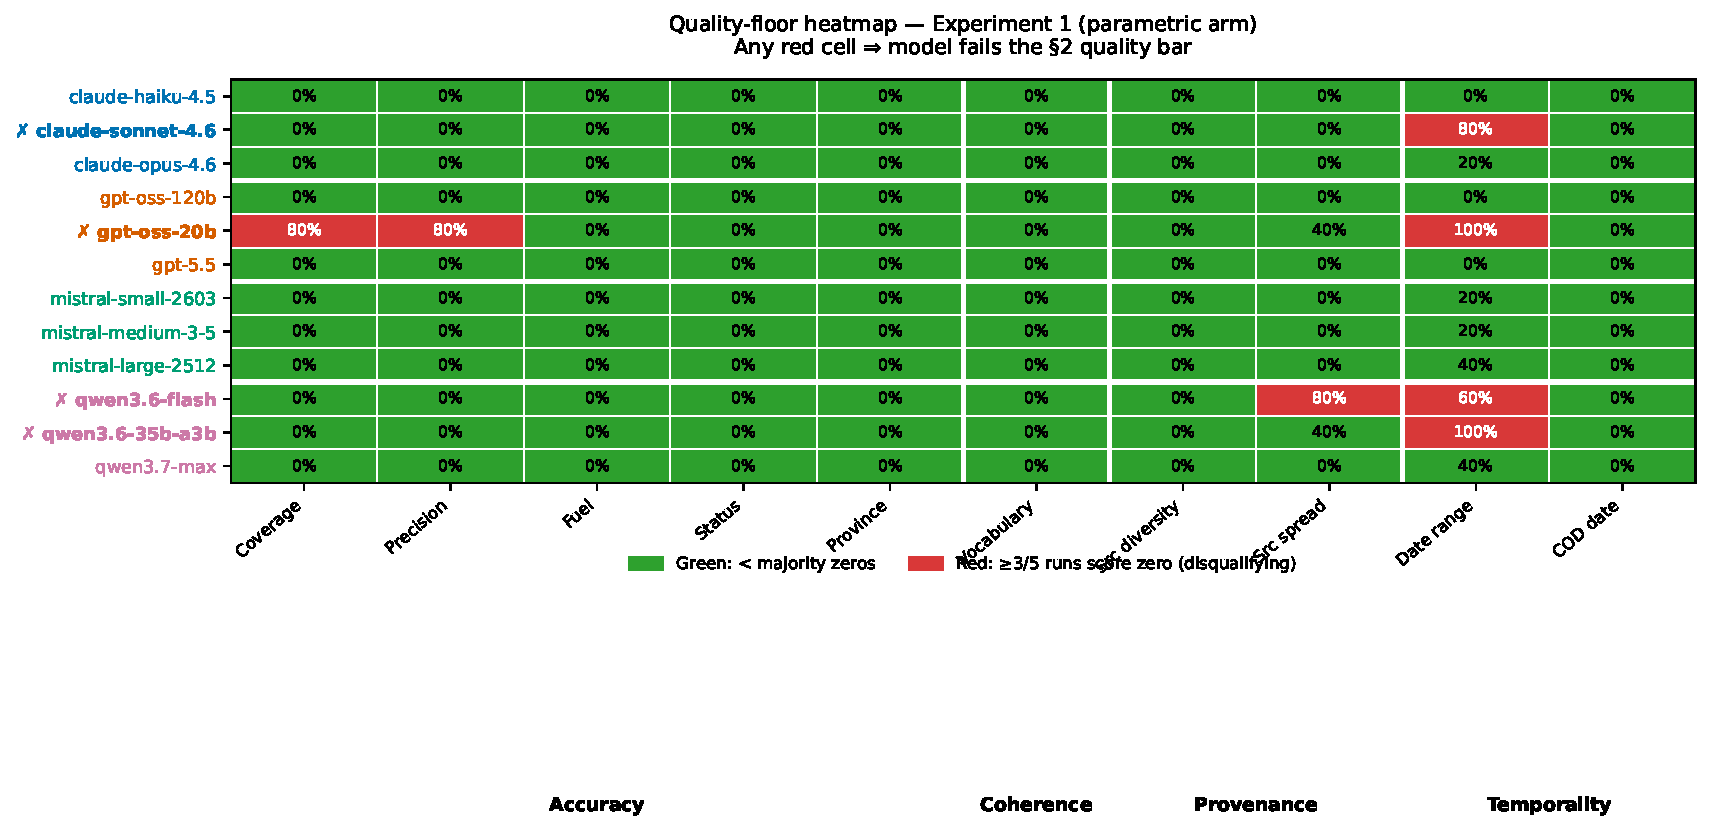
\includegraphics[width=\linewidth]{../../report/inputs/generated/fig_quality_floor_heatmap_exp1.pdf}
\caption{Per-criterion breakdown of the quality bar --- which dimension
each model fails. The bar is a conjunction, so a dark-red cell anywhere
in a column disqualifies that model. Quality-floor heatmap for
Experiment 1 (parametric arm, 14 models × 5 runs). Columns are the same
fourteen models as Figure~\ref{fig:direct-base}, laid out in the same
order --- architectural family (Claude, DeepSeek, GPT, Mistral, Qwen)
then size descending (larger first) --- with DeepSeek included. Rows are
the sub-score criteria, grouped by dimension and derived
programmatically from the scoring CSV. Only \textbf{discriminating}
sub-scores are shown: a criterion every model clears uniformly carries
no quality-floor signal and is dropped automatically when its
across-model spread falls below 0.1 (on the current data this drops
capacity sanity, core/capacity completeness, source presence,
dual-source, and as-of presence --- and with the latter rows, the whole
Field-completeness dimension). The surviving rows span Accuracy,
Coherence, Provenance, and Temporality. Each cell is the
\textbf{per-model mean} of that sub-score across the five runs, rendered
on a continuous red→green scale (0 = every run fails the criterion, 1 =
every run clears it); the simple mean suffices because a model that
systematically zeros a free criterion averages to ≈0 and reads dark red,
the §\ref{sec:quality} ``too weak to clear the bar'' signal. The
§\ref{sec:exp1} internal-coherence screen (the reference-free ρ=0.92
veto, \texttt{cap\_distinct\ ≤\ 4\ OR\ status\_distinct\ ≤\ 1}) is
\textbf{merged into the Coherence dimension} as its positive complement
(\texttt{1\ −\ veto}, the ``Internal coherence'' row), so higher is
better in lockstep with every other sub-score rather than occupying a
separate disqualifying column. The §\ref{sec:quality} quality bar is a
conjunction: a near-zero (dark red) cell anywhere in a model's column
means the bar is not cleared. Model labels are family-coloured and
dimension-separation lines isolate the criterion
groups.}\label{fig:quality-floor}
\end{figure}

\textbf{Reliability-gate sensitivity.} The Figure~\ref{fig:reliability}
grade depends on two tuning choices: the indicator set (which
reference-free dimensions enter the good-run conjunction) and the pass
threshold τ (a dimension counts as failed when its score is
≤ τ). The table below sweeps both --- three indicator sets ×
four thresholds --- and reports, for each cell, the number of
disqualified models (reliability \(\leq 1\)), whether that set equals
the baseline floor, and the Spearman correlation between reliability and
accuracy. The outcome barely moves across the grid: five models are
disqualified under the discriminating and all-reference-free sets at
every threshold, four (qwen3.6-flash escapes) under the narrower
coherence-only set, and the correlation stays at ρ = 0.78--0.80
throughout --- the headline reading of Figure~\ref{fig:reliability} does
not hinge on the gate's tuning. Source artifact:
\texttt{experiments/derived/exp1\_reliability\_sensitivity.csv}.

\begin{center}
% Generated by aedist.plot_exp1_reliability — do not edit.
\begin{tabular}{llrrcr}
\toprule
Indicator set & $n$ dims & $\tau$ & \#disqualified & = floor & Spearman $\rho$ \\
\midrule
Coherence only & 3 & 0.0 & 4 & no & 0.80 \\
 &  & 0.1 & 4 & no & 0.80 \\
 &  & 0.2 & 4 & no & 0.80 \\
 &  & 0.3 & 4 & no & 0.80 \\
\addlinespace
Discriminating & 6 & 0.0 & 5 & yes & 0.78 \\
 &  & 0.1 & 5 & yes & 0.80 \\
 &  & 0.2 & 5 & yes & 0.80 \\
 &  & 0.3 & 5 & yes & 0.78 \\
\addlinespace
All reference-free & 12 & 0.0 & 5 & yes & 0.78 \\
 &  & 0.1 & 5 & yes & 0.80 \\
 &  & 0.2 & 5 & yes & 0.80 \\
 &  & 0.3 & 5 & yes & 0.78 \\
\bottomrule
\end{tabular}

\end{center}

\textbf{Figure~\ref{fig:cost-quality} plotting detail.} In the
cost-vs-quality figure (Figure~\ref{fig:cost-quality}), each model
contributes a filled square at its pooled median true-positive count,
unfilled circles at every rep from the 2026-05-20 journal sweep, and ✕
markers at every rep from the 2026-05-21 reasoning-token top-up; the two
cohorts are pooled unconditionally (no canary gate), so intra-day
variability is absorbed into the reported within-model spread. Each rep
is plotted at its own per-call cost (cents USD, log scale), and a thin
polyline connects a model's reps in cost order. The Y axis starts at −5
so refusal markers at TP=0 sit visibly above the axis. Marker colour
encodes the architectural family from a colourblind-safe palette: Claude
(blue), GPT (vermillion), Mistral (bluish-green), Qwen (reddish-purple),
DeepSeek (orange). Per-model numbers backing the figure are written to
\texttt{report/inputs/generated/cost\_quality.csv} for audit.

\subsection*{Sweep configuration}
\addcontentsline{toc}{subsection}{Sweep configuration}

The sweep is defined in \texttt{experiments/experiments.toml} as
\texttt{sweep\_exp1\_baseline} (model\_set =
\texttt{modelset\_exp1\_journal}, repeat = 5, T = 0, seed = 42,
budget\_usd = 15, max\_tokens = 32768, prompt\_modules = []). These
match the Run-parameters table above and the as-run records in
\texttt{measurements.jsonl}
(\texttt{method\_params.max\_tokens\ =\ 32768}); an earlier draft quoted
the pilot's 8192-token / \$10 cap, which the journal sweep superseded.
Outputs land in \texttt{experiments/outputs/exp1/baseline/}; the prior
pilot runs are preserved under \texttt{baseline.pilot/}, kept separate
from the journal data. Results are ingested into
\texttt{measurements.jsonl} via \texttt{make\ rebuild-measurements}.

Experiment 1 was run as 5 reps per model on 2026-05-20 and topped up
with 3 additional reps per model on 2026-05-21 after a harness fix
restored capture of \texttt{reasoning\_tokens}. The top-up reps land in
\texttt{experiments/outputs/exp1/baseline.topup\_canary/} and
\texttt{baseline.topup/}; we pool them with the original five
unconditionally --- no canary gate. Intra-day variability across the two
acquisition windows is absorbed into the reported within-model spread
rather than filtered out.

\subsection*{What this experiment does and does not test}
\addcontentsline{toc}{subsection}{What this experiment does and does not test}

This experiment establishes the \emph{parametric ceiling}: the best
row-level quality achievable from model memory alone with a
well-specified prompt and no external information. It leaves three of
the four quality limits open: Coverage (facts absent from training
data), Freshness (facts post-dating training cutoff), and Coherence
(synthesis errors across the table). Only Articulation --- the gap
between intent and prompt --- is partially addressed by the structured
prompt. The gap between this ceiling and the quality bar defined in
§\ref{sec:quality} motivates the subsequent experiments.

\section{Experiment 2: Technical specification}\label{sec:annex-exp2}

\emph{This annex describes Experiment 2 as actually run. The registered
batch (protocol locked before dispatch) ran two arms, naive and
optimised, over the four agents below, N=5 per agent per arm, for 40
production sessions. Two further unregistered, exploratory conditions
(the same naive and optimised surfaces with a reference document pack
attached) were added during execution, bringing the corpus to 80 runs
and forming the 2×2 factorial (query mode × documents) reported in
§\ref{sec:exp2}'s Figure~\ref{fig:exp2-arms} and below. Row-level F1
against the reference was scored for all 80 runs (40 registered + 40
exploratory). Phase C cross-evaluation on the four §\ref{sec:quality}
dimensions is deferred to post-conference analysis. The full
registered-report write-up --- registration, the H1--H6 analysis plan,
execution deviations, and the descriptive statistics --- lives in the
technical report's Experiment 2 chapter; this annex pins only the as-run
specification and references that chapter for the inferential analysis.}

\subsection*{Task}
\addcontentsline{toc}{subsection}{Task}

Identify all thermal power plants in Vietnam using four state-of-the-art
cloud agents with extended reasoning and web access. Same target
population as Experiment 1: the \NumRefPlants-plant version-locked reference
inventory at
\texttt{data/reference/vietnam\_thermal\_plants\_v2\_classified.csv}.

\subsection*{Agents}
\addcontentsline{toc}{subsection}{Agents}

Four direct-API agents, ordered by ascending baseline smoke cost.
OpenRouter is not used here --- vendor-direct invocation keeps
web-search billing transparent.

\begin{longtable}[]{@{}
  >{\raggedright\arraybackslash}p{(\linewidth - 8\tabcolsep) * \real{0.2000}}
  >{\raggedright\arraybackslash}p{(\linewidth - 8\tabcolsep) * \real{0.2000}}
  >{\raggedright\arraybackslash}p{(\linewidth - 8\tabcolsep) * \real{0.2000}}
  >{\raggedright\arraybackslash}p{(\linewidth - 8\tabcolsep) * \real{0.2000}}
  >{\raggedright\arraybackslash}p{(\linewidth - 8\tabcolsep) * \real{0.2000}}@{}}
\toprule\noalign{}
\begin{minipage}[b]{\linewidth}\raggedright
\#
\end{minipage} & \begin{minipage}[b]{\linewidth}\raggedright
Vendor
\end{minipage} & \begin{minipage}[b]{\linewidth}\raggedright
Model
\end{minipage} & \begin{minipage}[b]{\linewidth}\raggedright
Country
\end{minipage} & \begin{minipage}[b]{\linewidth}\raggedright
Surface
\end{minipage} \\
\midrule\noalign{}
\endhead
\bottomrule\noalign{}
\endlastfoot
1 & Mistral & Mistral Large 2512 & FR & Agents API +
\texttt{web\_search} connector \\
2 & Alibaba & Qwen3-Max & CN & DashScope, \texttt{web\_search} inside
thinking mode \\
3 & OpenAI & GPT-5.5 & US & Responses API + \texttt{web\_search} +
reasoning \\
4 & Anthropic & Claude Opus 4.6 & US & Anthropic API +
\texttt{web\_search\_20250305} + adaptive thinking \\
\end{longtable}

Anthropic is pinned to Opus 4.6 (not 4.7) per the 2026-05-20 compose
decision: identical call shape, \textasciitilde40\% lower per-call cost
on the verified probe. Kimi K2.6 is disqualified --- vendor docs
document \texttt{thinking} and \texttt{\$web\_search} as mutually
exclusive, fatal for §\ref{sec:exp2}'s ``extended reasoning AND web
access'' requirement. Geographic / corpus spread (US × 2 + FR + CN) is
hypothesis-relevant: Chinese-language investor and trade documents on
Vietnamese power assets are under-indexed by Western search.

\subsection*{Baseline reference for cross-comparison}
\addcontentsline{toc}{subsection}{Baseline reference for cross-comparison}

The naive one-shot baseline that §\ref{sec:exp2} compares against is
\textbf{not} §\ref{sec:exp1}'s \texttt{modelset\_exp1\_journal} sweep.
It is the pre-existing \texttt{experiments/outputs/direct\_complete/}
artifact from \texttt{sweep\_direct\_complete} over
\texttt{modelset\_frontier\_10labs} --- a wider lab survey at a single
rep per model. Phase C will read from it directly; it is not re-run.

\subsection*{Phase structure}
\addcontentsline{toc}{subsection}{Phase structure}

\textbf{Phase A --- Reflexive prompt design (optimised arm).} Each agent
receives the baseline prompt
(\texttt{experiments/prompts/prompt\_complete.txt}), the four
§\ref{sec:quality} quality-dimension paragraphs verbatim, the task
statement, a JSON envelope spec, and the per-session budget cap
(announced upfront --- see ``Phase B dialogue policy'' below). The agent
is asked to return a fully-specified design --- \texttt{system\_prompt}
(threaded into the provider's system field at agent creation),
\texttt{designed\_prompt} (the user-side prompt sent on turn 1 of Phase
B), \texttt{settings} (\texttt{thinking}, \texttt{max\_tokens}), and
\texttt{rationale} --- that maximises the quality of the report it will
produce within the dual-axis session cap (below) and an overnight
wall-clock. Outputs land as
\texttt{<agent>\_phase\_a.json} with the four
envelope fields.

\textbf{Phase B-0 --- Single-rep smoke (optimised arm).} Each designed
prompt runs once (N=1) end-to-end through the multi-turn auto-reply loop
(see ``Phase B dialogue policy''). This is \emph{Test one before
blasting} applied at the experiment level: four outputs surface adapter
parser bugs, prompt failures, refusals, and real per-session cost before
committing the full N=5 batch. Gate to Phase B is a human review
confirming (i) all four adapters produced valid \texttt{RunRecord}
instances, (ii) parsed tables are non-empty, (iii) costs sit within the
dual-axis session cap empirically.

\subsubsection*{Phase B dialogue policy (fixed experimental condition)}
\addcontentsline{toc}{subsubsection}{Phase B dialogue policy (fixed experimental condition)}

Arms 2 and 4 are structured as a \emph{simple harness}: an LLM
orchestrator (the DeepSeek classifier) drives a loop in which the tested
LLM acts as the tool, with the harness state machine deciding which of
three fixed reply strings to send next. The word ``agentic'' applies to
this decomposition; it is ``simple'' in the sense that the orchestrator
issues fixed prompts rather than generating them adaptively, and the
loop logic is fully specified in code rather than delegated to a second
LLM's judgment.

After the Phase A design call, Phase B was a multi-turn conversation
against the same agent, driven by a small state machine. The author-side
reply was one of three fixed strings; the choice was made after each
agent response by a one-shot LLM classifier deciding whether the agent
had ``produced a report'' or not. The classifier's cost was harness
overhead and was \emph{not} deducted from the SOTA agent's session
budget. The as-run classifier was \texttt{deepseek/deepseek-v4-pro}; the
registered --- and earlier-run --- choice was
\texttt{nvidia/nemotron-nano-9b-v2}, with \texttt{mistral-small-latest}
confined to the pilot. DeepSeek is a third-party vendor distinct from
all four subjects (Anthropic, OpenAI, Mistral, Alibaba), so the
classifier never formed a same-vendor self-evaluation pair with the
agent it judged --- the cross-vendor independence the registration
sought when it moved off the original same-vendor classifier.

Three reply strings, verbatim:

\begin{itemize}
\tightlist
\item
  \textbf{ENCOURAGE} (sent up to three times before forcing terminal):
  \emph{``Proceed as you think is best in autonomous agentic mode.''}
\item
  \textbf{VERIFY} (sent exactly once after the first agent response
  classified as a report): \emph{``Thank you for the inventory. Please
  now verify and polish it in ONE focused pass, prioritising: (a)
  per-row provenance --- every Source 1 and Source 2 cell must point to
  a specific URL from your bibliography; (b) coverage --- any plant
  present in your bibliography but absent from the table; (c)
  temporality --- every row has an as-of date or status-change note; (d)
  internal consistency --- capacity totals reconcile across the table
  and the statistical summary. Return the corrected inventory only ---
  no meta-commentary on what you changed.''}
\item
  \textbf{TERMINAL} (sent when remaining budget ≤ 20\% of the cap, or
  after three consecutive \texttt{no\_report} classifications ---
  ENCOURAGE on the first two, TERMINAL on the third): \emph{``I have no
  additional directive to give you. Please proceed to generating the
  report without further asking. If you cannot, we would appreciate to
  know why, but the discussion will stop here in any case. Thanks for
  your understanding.''}
\end{itemize}

Every user-side message after turn 1 carries a chat-text status prefix
--- \emph{``Status: remaining X.XK of 50K tokens, \$X.XX of \$3.00.
Wall-clock elapsed Ys. Verify .''} --- exposing both budget axes to the
agent, and, where the provider exposes a metadata surface, a structured
metadata field carrying \texttt{cap\_tokens} and \texttt{cap\_usd}.
After VERIFY's response is captured (or after TERMINAL's response), the
loop terminates.

\textbf{Phase B --- Execution (N=5).} Gated on a clean B-0 review. Each
designed prompt runs five times against a single provider per agent (the
closed-weight frontier agents have one vendor each; the cross-provider
variance reported for MoE models in \ref{sec:annex-exp1} does not
apply). The four Phase B-0 sessions are the first reps of these five.

\subsection*{Arms and budget}
\addcontentsline{toc}{subsection}{Arms and budget}

The registered design has two arms over the same four agents, five reps
each (40 production sessions):

\begin{itemize}
\tightlist
\item
  \textbf{Naive arm} --- Doc-07
  (\texttt{experiments/sota/protocol\_07\_naive\_prompt.md}) sent
  verbatim as the sole user message, no system prompt, web search on,
  one model response per session. This carries the v2 task statement and
  quality criteria but none of the optimised arm's methodology (budget
  rules, planning headroom, source admissibility, calibrated confidence
  vocabulary). It is the null comparator: the contrast between arms
  isolates the protocol scaffolding's contribution. The file at this
  path was revised after all naive-arm sessions had run (2026-05-24):
  the five anthropic-direct run records archive the as-sent user
  message --- the earlier, shorter version, identical across runs ---
  and the three web-product sessions (2026-05-22--23) predate the
  revision, though their session records do not archive the sent
  prompt. The expanded current version is the Experiment 1
  analysis-cohort prompt reproduced in \ref{sec:annex-exp1}.
\item
  \textbf{Optimised arm} --- Phase A design call followed by the Phase B
  multi-turn state machine above (Phase B-0 then Phase B-full).
\end{itemize}

Both arms share one \textbf{dual-axis per-session budget cap: 50 000
tokens \emph{or} a \$3 dollar guard, whichever fires first triggers
TERMINAL.} Dollar-only caps disadvantage models with expensive output
tokens; the token cap binds reasoning capacity comparably across vendors
while the dollar guard binds total bill. The cap is the experimental
condition --- no session is dropped for cost or wall-time reasons. The
realised per-session and per-batch costs are reported in
§\ref{sec:exp2}'s Figure~\ref{fig:exp2-arms} and the technical report
chapter, not pinned here.

\subsection*{As-run deviations from the registration}
\addcontentsline{toc}{subsection}{As-run deviations from the registration}

The experiment was pre-registered (protocol locked before the production
batch, with an H1--H6 analysis plan). Execution deviated from the
registration in three headline ways, all reported candidly rather than
hidden:

\begin{itemize}
\tightlist
\item
  \textbf{A documents axis was added.} Beyond the two registered arms,
  two further \emph{unregistered, exploratory} conditions --- the same
  naive and optimised surfaces with a reference document pack attached
  --- were run, expanding the corpus from 40 to 80 sessions and forming
  the 2×2 factorial (query mode × documents) of §\ref{sec:exp2}'s
  Figure~\ref{fig:exp2-arms}. These two conditions are exploratory by
  construction: they are never aggregated with the two registered arms.
\item
  \textbf{Claude's optimised arm is excluded from the
  bibliography-quality table (0 of 5 runs).} None of Claude's five
  optimised-arm sessions yielded a bibliography parseable by the
  structure analyser, so the cell is blank in the bibliography-quality
  table. This is a \emph{bibliography-parsability} exclusion only: those
  same five sessions remain row-level-F1-scorable (N=5) via the LP
  matcher, and they are present in the 2×2 F1 table. The 0/5 must not be
  read as the runs failing outright.
\item
  \textbf{Phase C cross-evaluation is deferred.} The four-dimension peer
  cross-evaluation was reserved for post-conference analysis; the as-run
  results below and in §\ref{sec:exp2} are the operational and F1-based
  metrics, not the §\ref{sec:quality}-dimension cross-eval scores.
\end{itemize}

The registered-report treatment of these --- the locked H1--H6 plan,
per-arm validity and exclusion criteria, and the descriptive F1/cost
statistics --- is in the technical report's Experiment 2 chapter; this
annex does not reproduce those statistics.

\subsection*{Harness}
\addcontentsline{toc}{subsection}{Harness}

This experiment is script-based, not sweep-based. No
\texttt{sweep\_exp2\_*} block exists in
\texttt{experiments/experiments.toml}. Implementation surface:

\begin{itemize}
\tightlist
\item
  \texttt{src/aedist/adapter\_mistral.py} --- Mistral Agents API adapter
  (multi-turn continuation + 5xx retry).
\item
  \texttt{src/aedist/adapter\_qwen\_dashscope.py} --- DashScope adapter
  (multi-turn continuation).
\item
  \texttt{src/aedist/adapter\_openai\_responses.py} --- OpenAI Responses
  adapter (multi-turn continuation).
\item
  \texttt{src/aedist/query\_anthropic.py} --- Anthropic adapter
  (multi-turn continuation).
\item
  \texttt{experiments/sota/exp2\_interactive\_smoke.py} --- author-side
  harness running Phase A + Phase B state machine.
\item
  \texttt{experiments/sota/dialogue\_classifier.py} --- one-shot LLM
  classifier deciding \texttt{report} vs \texttt{no\_report}.
\item
  \texttt{experiments/outputs/sota\_smoke/} and
  \texttt{sota\_exp2\_smoke/} --- artifact directories. Each Phase B
  turn writes
  \texttt{<agent>\_turn\_NN.\{user.txt,raw.json,record.json,cost.json,classification.json,report.md,citations.json\}}.
\item
  \texttt{experiments/derived/tab\_exp2\_2x2.csv},
  \texttt{report/inputs/generated/tab\_exp2\_bib\_quality.tex} ---
  as-run derived tables (2×2 F1/cost factorial; per-arm bibliography
  quality). The \texttt{experiments/derived/sota\_cross\_eval.csv} Phase
  C target is reserved for the deferred cross-evaluation.
\end{itemize}

\subsection*{Evaluation}
\addcontentsline{toc}{subsection}{Evaluation}

Phase B outputs are evaluated against the \NumRefPlants-plant reference using the
same \texttt{src/aedist/evaluate.py} machinery as §\ref{sec:exp1} (LP
matcher, ADR-2/3, \texttt{similarity\_threshold\ =\ 90},
\texttt{capacity\_weight\ =\ 0.001}), yielding row-level F1 and
per-attribute accuracies. Phase C cross-evaluation --- peer scoring of
each output on the four §\ref{sec:quality} dimensions --- is deferred to
post-conference analysis; the as-run results are the F1-based and
operational metrics of §\ref{sec:exp2}, not the
§\ref{sec:quality}-dimension cross-eval scores.

\subsection*{What this experiment does and does not test}
\addcontentsline{toc}{subsection}{What this experiment does and does not test}

This experiment tests whether removing the §\ref{sec:exp1} handicaps (no
web, no tools, no documents), by handing the task to a commercially
available deep-research surface, clears the §\ref{sec:quality} quality
bar. It does not test custom workflows or local models; that is
§\ref{sec:fusion}. It does not test how the four dimensions trade off
under a fixed budget; that is §\ref{sec:fusion} once the
composite-quality scorers exist. It does not test browser-automated
surfaces (ChatGPT.com, Claude.ai chat UI) --- only direct vendor APIs.

\textbf{Wikipedia/Wikidata compliance.} Because a derivative of the
reference dataset was published on Wikipedia before the experiment, the
experimental protocol bans Wikipedia, Wikidata, DBpedia, and mirrors as
admissible sources --- the risk is both training-data and web-search
contamination. We audited compliance mechanically: URL-domain matching
over every Source 1 and Source 2 cell and every bibliography entry of
all 40 registered runs. We detected banned-domain citations in 5 of the
20 optimised-arm runs, concentrated in Mistral (runs 1--4) and OpenAI
(run 1); we did not detect banned-domain citations in the Anthropic or
Qwen optimised runs. In the naive arm, where the prompt carries no
source ban, 1 of the 20 runs (OpenAI run 5) cited a banned domain. This
audit is mechanical only: paraphrased Wikipedia content without a URL is
not detected.

\section{Supplementary figures}\label{sec:annex-suppfigs}

\begin{figure}
\centering
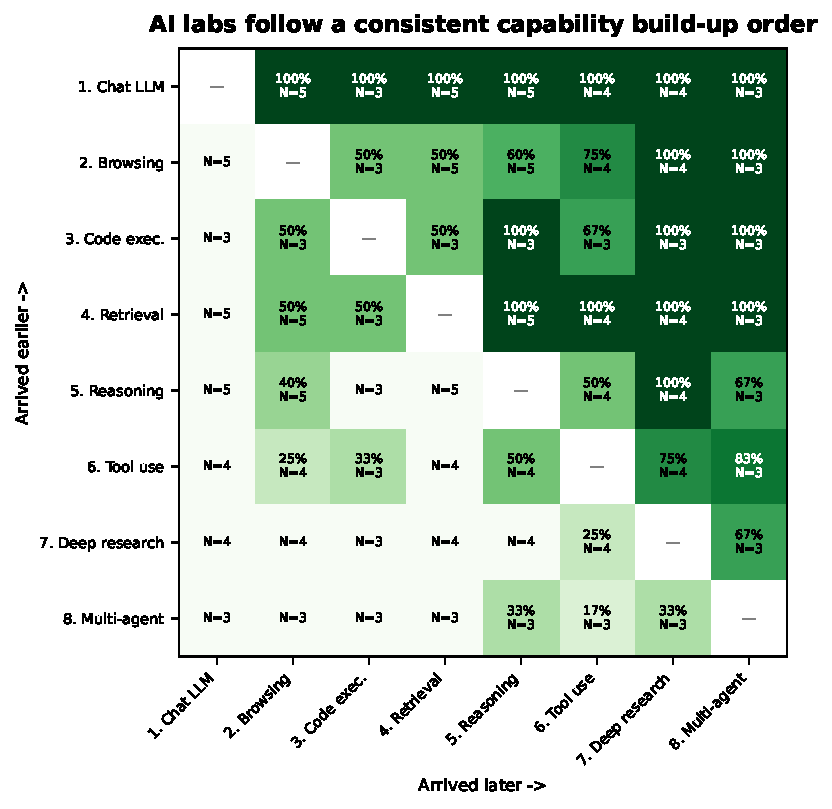
\includegraphics[width=\linewidth]{../../report/inputs/generated/fig_capability_dag.pdf}
\caption{Empirical capability transition matrix across N=5 labs. Each
cell shows the fraction of labs where feature i (row) shipped before
feature j (column), conditional on both being present; N per cell. Ties
split as 0.5 so symmetric pairs sum to 100\%. White = no lab made that
transition; dark green = all labs did. Features 3 and 4 (code execution
× retrieval) emerge in parallel. Feature 5 (reasoning) consistently
follows features 1--3. Feature 7 (deep research) draws on features 2 and
5. Descriptive historical record, N=5 labs --- no statistical
inference.}\label{fig:capability-dag}
\end{figure}

\begin{figure}
\centering
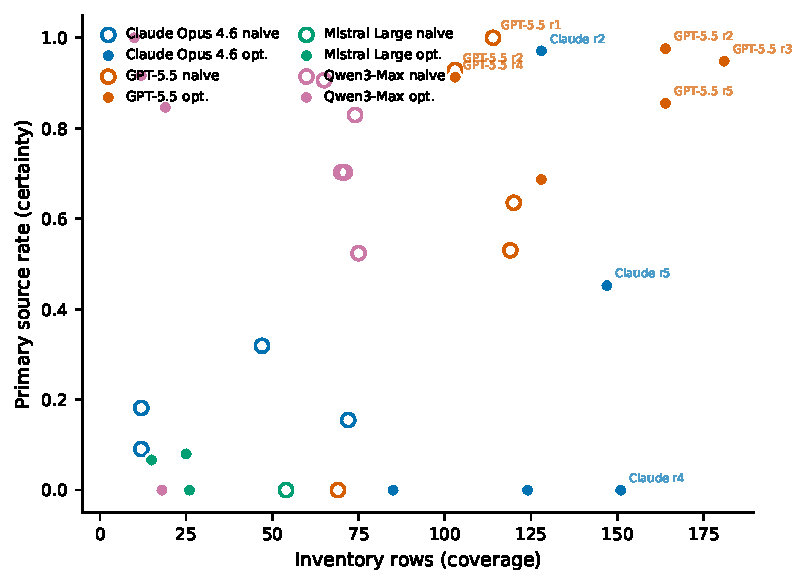
\includegraphics[width=\linewidth]{../../report/inputs/generated/fig_exp2_coverage_certainty.pdf}
\caption{Only one agent combines broad coverage with systematic
double-sourcing. Coverage vs.~corroboration across 31 Exp2 runs (9 with
zero parsed inventory rows excluded: Mistral arm 2 all 5 runs, Anthropic
arm 2 runs 2/4/5, and Anthropic arm 1 run 4). X-axis: inventory rows
enumerated. Y-axis: rows with a Source 2 citation present. The dashed
diagonal marks full double-sourcing (every row corroborated). Filled
diamonds: optimised arm (arm 2); open circles: naive arm (arm 1).
Colours encode agents. OpenAI optimised alone sustains high values on
both axes; Anthropic optimised shows a corroboration ceiling despite
growing coverage; Qwen clusters near the diagonal at low
volume.}\label{fig:coverage-certainty}
\end{figure}

\section{Experiment 1: per-plant recognition matrix and the status composition of task difficulty}\label{sec:annex-recognition}

Figure~\ref{fig:recognition-matrix} places each of the \ExpOneMatrixPlants{} reference
plants on its own row (names read left-to-right, no rotation) against
the \ExpOneMatrixRuns{} Experiment 1 runs (14 models × 5 repetitions) as columns. A blue
cell marks a recognised plant (true positive); an empty cell, a miss.
Rows are grouped by status, then by decreasing capacity, using the same
status categories as the difficulty table below. To keep plant names
legible at print scale, the matrix is split across pages by lifecycle
stage. A final page lists the \ExpOneMatrixFPs{} most frequent false positives across
all runs, sorted by decreasing occurrence, in red --- the paper's
false-positive convention (unmatched: extracted but not in the
reference; possibly real, not necessarily fabricated). Unlike
Figure~\ref{fig:direct-base}, which only counts each run's recognised
plants, the fixed-row alignment reveals \emph{which} plants each model
misses: famous plants form dense rows, obscure ones sparse rows.

\refstepcounter{figure}\label{fig:recognition-matrix}
\noindent\emph{Figure \thefigure. (Next three pages.) Experiment 1 recognition
matrix, transposed to portrait so plant names stay legible: the \ExpOneMatrixPlants{} reference
plants are rows (grouped by status, then by decreasing capacity, with the status
bands labelled in the right margin) and the \ExpOneMatrixRuns{} runs (14 models × 5 repetitions)
are columns under a three-level family / version / repetition header, in
Figure~\ref{fig:direct-base}'s order: family, then decreasing effective parameter
count. Blue = plant recognised. Pages 1--2 split the plants by lifecycle stage
(operational, retired, and cancelled plants, then proposed, planned, and
under-construction ones); page 3 lists the \ExpOneMatrixFPs{} most frequent false positives
(red).}
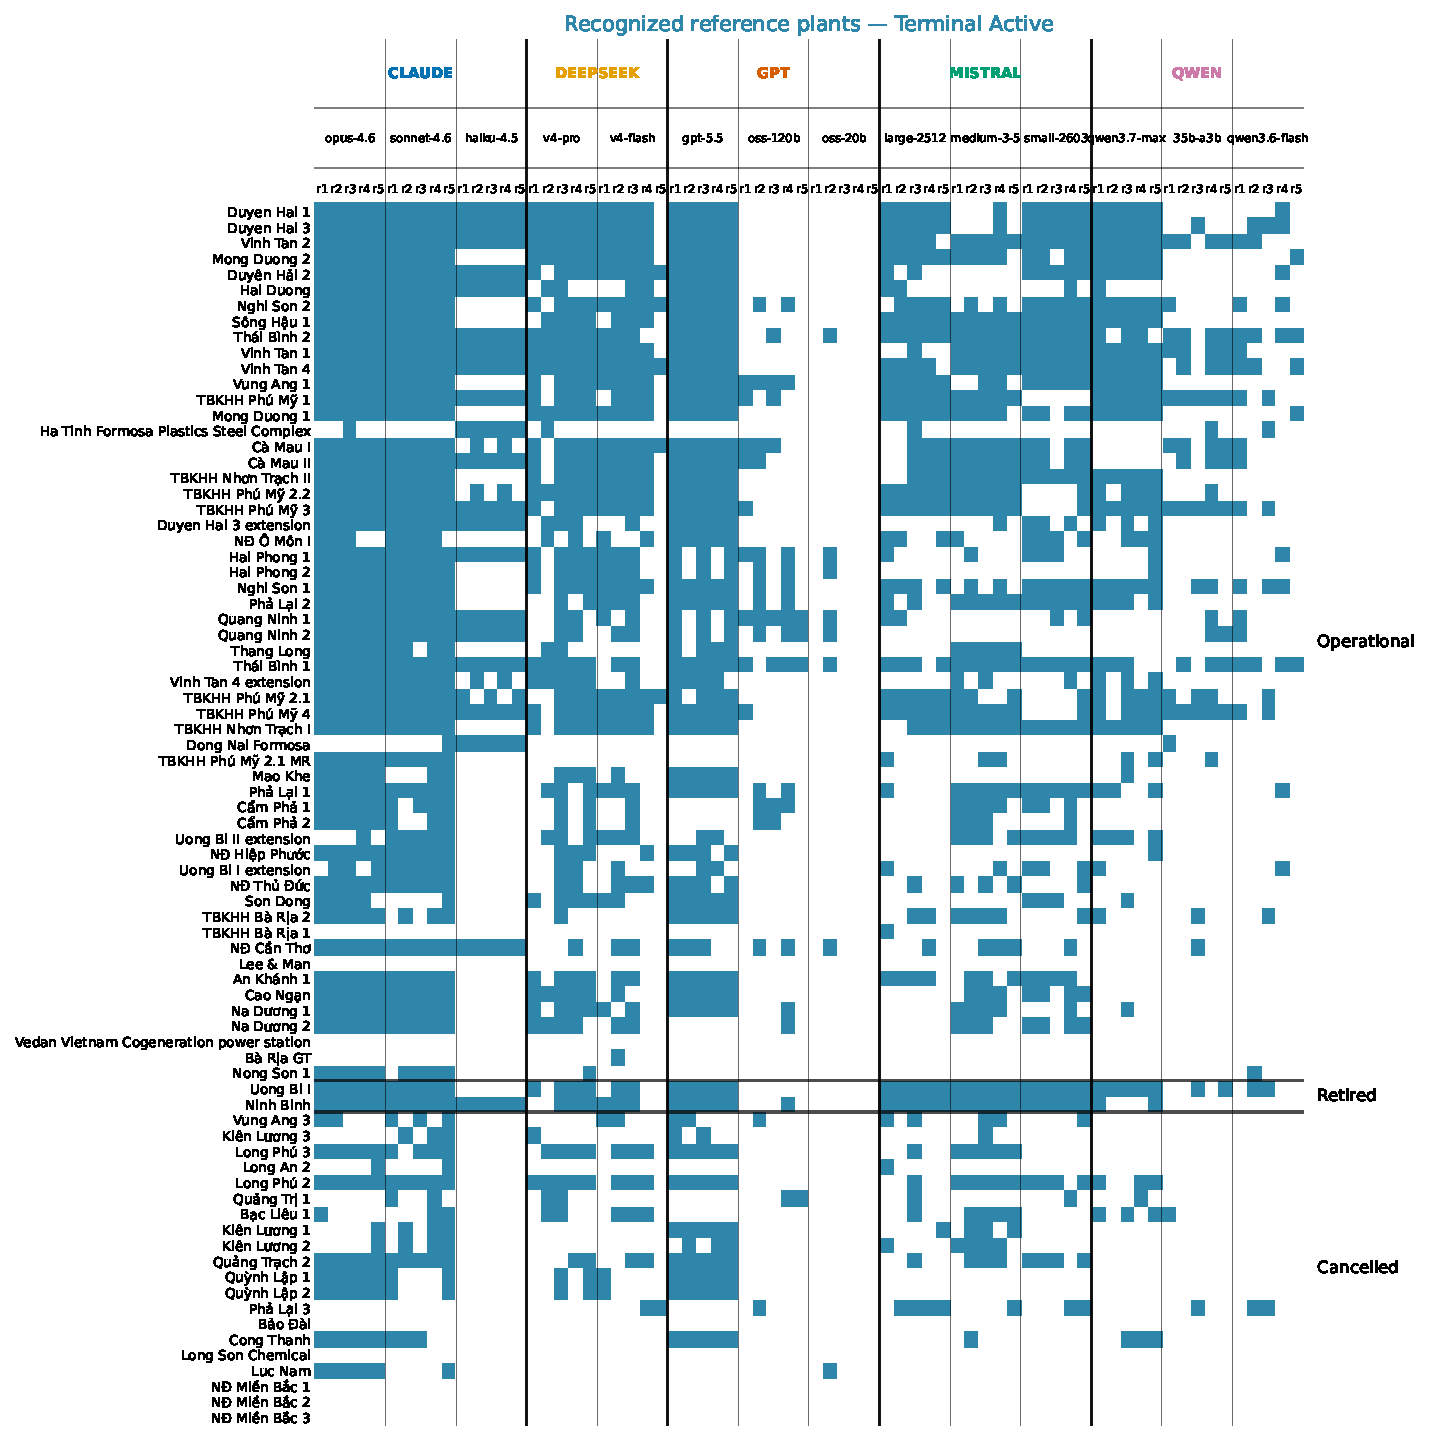
\includepdf[pages=-,pagecommand={\thispagestyle{plain}}]{../../report/inputs/generated/fig_exp1_recognition_matrix_portrait.pdf}

The table below shares the same data derivation as the figure (library
\texttt{aedist.exp1\_recognition} --- common cause, no
producer--consumer chaining) and decomposes the difficulty by status.
The reference list is dominated by proposed plants --- the largest share
--- which parametric memory cannot know; their mean recognition rate is
far below that of operational plants. The low overall recognition is
therefore structural, a property of the list's composition, not merely a
model failure.

\begin{table}[htbp]
\centering
\caption{\label{tbl:status-difficulty}Composition of the reference list
by status, and mean recognition rate (Experiment 1, direct method: 14
models × 5 repetitions). The rate is the share of run × plant cells
recognised among plants of that status.}
% Auto-generated by aedist.tabulate_status_difficulty — do not edit
\begin{tabular}{@{}lrrr@{}}
\toprule
Status & n & Share of list & Recognition rate \\
\midrule
Proposed & 68 & 38.4\% & 8.1\% \\
Planned & 21 & 11.9\% & 30.3\% \\
Under construction & 10 & 5.6\% & 45.3\% \\
Operational & 56 & 31.6\% & 46.6\% \\
Retired & 2 & 1.1\% & 63.6\% \\
Cancelled & 20 & 11.3\% & 16.9\% \\
\midrule
\textbf{All} & \textbf{177} & \textbf{100.0\%} & \textbf{26.6\%} \\
\bottomrule
\end{tabular}

\end{table}

\section{Run-grain screen validation: within-model accuracy gap}\label{sec:annex-screen}

The §\ref{sec:discussion} Discussion paragraph ``Internal coherence as a
zero-reference screen'' reports a pooled Spearman ρ = 0.92 between
within-run capacity variability and reference-based F1 across 70
Experiment 1 runs. A potential confound: weak models are weak across the
board, so the correlation may reflect \emph{model quality} rather than
run quality --- the screen may be near-tautological at the model grain.
This annex tests whether the screen discriminates good from bad runs of
the \textbf{same model}, removing the across-model confound.

\textbf{Method.} For each of the 70 runs (14 models × 5 repetitions), we
compute \texttt{cap\_distinct} (number of distinct capacity values in
the raw output table) and \texttt{status\_distinct} (number of distinct
status values) directly from the exp1\_batch2 raw CSVs. The veto rule
\texttt{cap\_distinct\ ≤\ 4\ OR\ status\_distinct\ ≤\ 1} assigns each
run to vetoed or surviving. Reference-based F1 is taken from the
cross-evaluation CSV (the \emph{outcome}; it is never used as a veto
input, preserving the reference-free property of the screen). The
model-stratified Kendall τ counts concordant and discordant pairs
of \texttt{(cap\_distinct,\ F1)} \emph{only within each model's 5 runs},
then sums the counts across all 14 models --- an exact removal of the
across-model confound.

\textbf{Results.} The model-stratified Kendall τ of cap\_distinct
vs F1 is \textbf{+\ScreenTauCap} (\ScreenTauCapConcordant{} concordant, \ScreenTauCapDiscordant{} discordant pairs across \ScreenNModels{}
models; \ScreenPositiveSpearman/\ScreenNModels{} models show a positive within-model Spearman ρ). For
status\_distinct vs F1 the stratified τ is \textbf{+\ScreenTauStatus} (\ScreenTauStatusConcordant{}
concordant, \ScreenTauStatusDiscordant{} discordant). Across-model pooled statistics (tautological
baseline): mean F1 of vetoed runs = \ScreenPooledVetoedMeanFOne{}, surviving = \ScreenPooledSurvivingMeanFOne{}, gap =
+\ScreenPooledGap{}. Within-model binary gap (only the \ScreenNMixed{} models with both vetoed and
surviving runs): mean of per-model gaps = \textbf{+\ScreenBinaryGap} (\ScreenPerModelGaps). The reduction from
the pooled gap (+\ScreenPooledGap) to the within-model gap (+\ScreenBinaryGap) shows that
roughly half the pooled signal was attributable to the across-model
confound; the residual within-model effect (+\ScreenBinaryGap) is the honest lower
bound.

\textbf{Interpretation and limitations.} The within-model directional
signal is positive and consistent across a clear majority of models
(\ScreenPositiveSpearman/\ScreenNModels), supporting the claim that the screen earns its keep at the run
grain. However, the statistic is modest, and only \ScreenNMixed{} of the \ScreenNModels{} models
have both vetoed and surviving runs --- the binary within-model
comparison is therefore underpowered for formal significance testing.
One false-veto case exists: \ScreenFalseVetoModel{} run \ScreenFalseVetoRun{} (F1 = \ScreenFalseVetoFOne)
is vetoed by the cap\_distinct threshold yet outscores one of the
model's two surviving runs. These limitations are acknowledged; the
screen is presented as an existence proof validated within-model, not as
a fully calibrated detector. The cutoff thresholds were tuned in-sample
on the same 70 runs --- cross-validation against Experiment 2 or
held-out runs is future work.

\emph{Supporting data:
\texttt{report/inputs/generated/tab\_screen\_validation\_within\_model.csv}
(produced by \texttt{src/aedist/screen\_validation\_within\_model.py},
wired in \texttt{experiments/render.mk}).}

\section{Capability rollout: per-lab shipping order}\label{sec:annex-rollout}

This annex records the detailed shipping-order observations behind
Figure~\ref{fig:capability-timeline}, kept out of the
§\ref{sec:capability} body to keep the capability discussion at the
level of the envelope framing. The figure is descriptive: no claim is
made that any lab is ``ahead'' or that the feature order is forced.

\textbf{Feature sequence and cross-lab parallelism.} Features 1 through
4 ship within \textasciitilde24 months across the industry, with the
first three (chat LLM, browsing, code execution) arriving at OpenAI
between late 2022 and mid-2023 before retrieval followed in October
2023. Features 3 and 4 emerge in parallel across labs: the per-lab order
varies (Anthropic shipped retrieval before code execution; OpenAI the
reverse; Mistral the same day), and the \emph{cross-lab} shipping
windows overlap substantially. Feature 3 (code execution) was the
earliest tool-use surface shipped as a built-in consumer feature,
predating the general MCP-like surface of feature 6 by \textasciitilde18
months at OpenAI. Feature 7 (deep research) draws on both features 2 and
5 --- at every lab where it shipped as a product, deep research arrived
within 1--5 months of having both browsing and reasoning in place. This
is structural evidence that the order is observed in the data, not
imposed by the framing.

\textbf{The DeepSeek negative case.} DeepSeek confirms the
framework-not-model framing: it ships features 2 and 5 (Internet Search
in V2.5; R1 reasoning) and the model components that would enter a
deep-research loop (V3.1's search-agent claims, V3.2's
thinking-in-tools), but has not packaged the composer as a public
product within the cutoff --- capability components present, product
surface absent.

\textbf{Two axes absent by construction.} The figure goes quiet after
mid-2025 because leading labs had filled all eight features, not because
development stalled: context length, shell-level execution, persistent
agent scaffolds, and the modality axis --- text to vision to real-time
audio --- all continued to advance outside the tool-affordance ladder
this schema tracks. Two further dimensions are absent by construction.
The \emph{constraint axis} --- refusal training, content policy, and
red-teaming --- shaped which requests these consumer products would
serve, running alongside the capability expansion the figure shows but
perpendicular to it. And the consumer-product methodology excludes the
military and dual-use deployment track: a parallel trajectory operating
at comparable capability levels, now routine front-page news, that the
commercial-product framing does not capture and does not claim to.

\section{Aggregation sweep and vote gate}\label{sec:annex-fusion}

This annex develops the fusion material summarised in
§\ref{sec:fusion}. Pooling the \ExpOneNRuns{} parametric-baseline runs from
§\ref{sec:exp1} (\ExpOneNModels{} models × 5 repetitions) treats each run as a noisy
partial observer of the \NumRefPlants-plant reference: the per-plant recognition
matrix (\ref{sec:annex-recognition}) shows that the operational core
forms dense rows while proposed plants form sparse ones, and the
density profile predicts which plants are structurally recoverable by
pooling alone. The paragraphs below first draw the design consequence
of the single-model ceiling, then quantify what run-level fusion
already delivers.

The single-model ceiling motivates a stateful architecture --- one that
keeps an organised memory between runs instead of starting from scratch
at each prompt. The equalisation result in §\ref{sec:exp2} sharpens the
target: once the agents share a good document set, single-shot
performance converges and the binding constraint appears to shift from
model capability to document quality. The value is therefore in the corpus
and the sourcing process --- assembling, curating, and resolving the
documents --- rather than in chasing a stronger model. That is precisely
what a stateful pipeline invests in: a managed, auditable knowledge base
rather than a one-shot prompt against whatever model is current. The
§\ref{sec:quality} quality dimensions measure \emph{output}: accuracy,
coherence, provenance, temporality. A targeted pipeline adds a second
axis, \emph{method quality}: whether the process is auditable,
reproducible, and cost-predictable independent of which model runs it.
Such a system is stateful: it maintains a sourced narrative knowledge
base, where each asset record carries its full lifecycle history and
conflict-resolution record. The statistical table is a derived
projection --- a snapshot at a reference date --- from the narrative
inventory rather than a direct model output. Each cell is a claim,
recording its source, date, confidence, and conflict-resolution history.
The narrative layer carries the temporal dimension deferred in
§\ref{sec:quality}: plant lifecycle events, PDP-cycle reclassifications,
developer changes, and contested status periods are recorded as
annotated history rather than as overwritten state.

Each cell in a power-plant inventory (one plant, one attribute, one
value) maps to a knowledge-graph triple: subject, predicate, object.
Fusing tables from competing sources is therefore the same problem as
fusing overlapping triple sets, with the same need for conflict
resolution, source authority, and temporal versioning. Cases that
rule-based schema-fixed systems cannot handle cleanly --- assets
mid-lifecycle, contested sources, multilingual records, conditional
projections --- are where language-model reasoning adds genuine value.

\textbf{Pooling runs by simple union more than doubles recall relative
to the single-run mean (\AggUnionGainX×), at no new collection cost.} The 14-model exp1\_batch2 cohort (a subset of the
16-model Experiment 1 sweep, dropping \texttt{qwen3.6-27b} and
\texttt{qwen3.6-plus}; see the cohort note in §\ref{sec:exp1}) allows a
controlled evaluation of pooling recipes without any new API calls: a 4
× 3 × 4 factorial sweep. The sweep crosses four merge methods (union;
majority at \(k\)=2 and \(k\)=3; confidence-weighted), three pool sizes
(2, 3, 4), and four diversity rules (intra-model; cross-model selecting
the cheapest, most expensive, or alternating models by run cost),
scoring each aggregated list against the \NumRefPlants-plant reference using the
same LP matcher as §\ref{sec:exp1}. Union aggregation dominates as a
\textbf{recall} lever across all diversity rules and pool sizes: the
best union recipe, three runs from the three most expensive models,
achieves recall = \AggBestUnionRecall{} at a combined cost of \$\AggBestUnionCost{}, compared to a
single-run mean recall of \AggSingleRunMeanRecall{}. This is a \AggUnionGainX× improvement over the
mean, though it remains below the best individual run's recall (\AggBestSingleRecall{}
for claude-sonnet-4.6) because precision falls as the union list grows
(\AggBestUnionCandidates{} candidate plants for \NumRefPlants{} reference plants). F1 for the best union
cell (\AggBestUnionFOne) is slightly below the best single-run F1 (\AggBestSingleFOne); union
buys coverage breadth at a precision cost, not a free F1 gain. Majority
voting and confidence-weighting both reduce recall relative to union at
every pool size, because the Experiment 1 vocabulary is rich enough that
most true plants appear in at most one run in any given pool; a majority
gate filters them out. Intra-model pooling (averaging over the 14
models) reaches recall = \AggIntraPoolThreeRecall{} at pool size 3 for \$\AggIntraPoolThreeCost{}, a practical
option when budget constrains the model set. The cross-model-low recipe
(cheapest models only) performs poorly (recall ≈ \AggLowRecallMin--\AggLowRecallMax), confirming
that marginal plant recall is concentrated in the frontier models. These
results do not update the headline F1 from §\ref{sec:exp1}, which
reports per-model single-run performance for comparability with existing
benchmarks; they establish that cross-model union is the recommended
aggregation recipe for practitioners targeting maximum coverage at a
fixed token budget. Source artifact:
\texttt{experiments/derived/aggregation\_sweep.csv}.

\textbf{Requiring two models to agree nearly eliminates false
positives.} Restricting the pool to the four frontier models and
applying a simple ≥2-models presence rule --- a plant is admitted if at
least two of the four models name it --- sharpens the precision/recall
trade-off in both experiments (Figure~\ref{fig:fusion-mvp}). Applying the rule separately to
Experiment 1 (the same four models, answering from memory, × 5 repeats)
and the Experiment 2 naive arm (E1 vs E2) gives: under ≥2-models in E1,
F1 = \FusionRTwoEOneFFrac{} (TP = \FusionRTwoEOneTP, FP = \FusionRTwoEOneFP); under ≥2-models in the E2 naive arm, F1
= \FusionRTwoETwoOneDFFrac{} (TP = \FusionRTwoETwoOneDTP, FP = \FusionRTwoETwoOneDFP). The vote gate trades a little recall for a
large precision gain, the mirror image of the union recipe above.
Source artifact: \texttt{report/inputs/generated/fusion\_mvp.csv}.

\begin{figure}
\centering
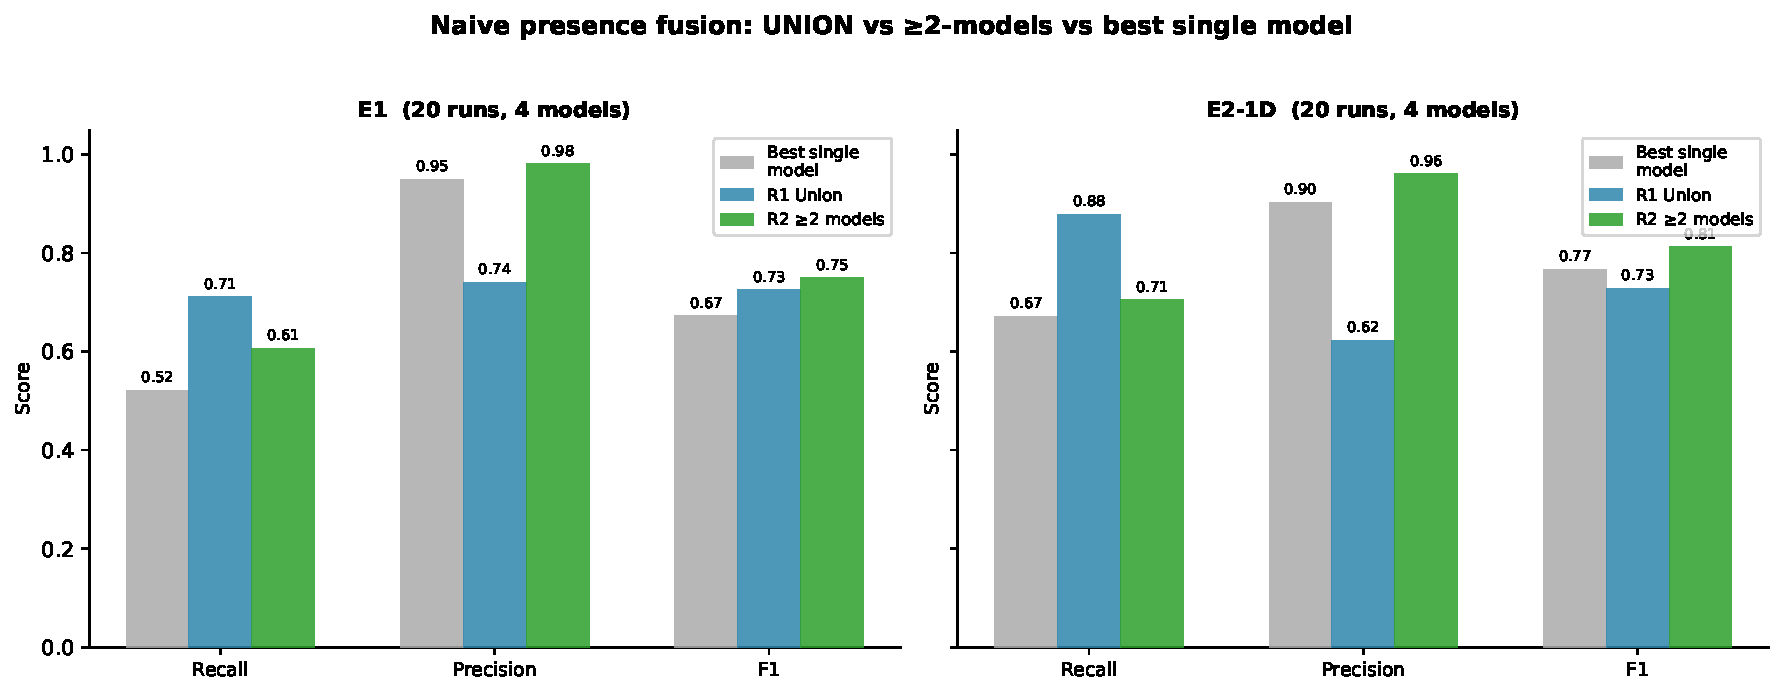
\includegraphics[width=\linewidth]{../../report/inputs/generated/fig_fusion_mvp.pdf}
\caption{A two-model agreement rule buys precision cheaply: \FusionRTwoEOneTP--\FusionRTwoETwoOneDTP{}
confirmed plants against \FusionRTwoEOneFP--\FusionRTwoETwoOneDFP{} false positives, with no new API calls.
Naive presence fusion across the 4-frontier-model Experiment 1 cohort
and Experiment 2 naive arm (N=20 runs each: 4 models × 5 repeats). Top
panel (E1 parametric): UNION and ≥2-models fusion rules vs best single
model. Bottom panel (E2 naive arm): same rules. TP = plants matched
against the reference; FP = unmatched plants (extracted but not in the
reference). Under ≥2-models in E1: F1=\FusionRTwoEOneFFrac{}, TP=\FusionRTwoEOneTP, FP=\FusionRTwoEOneFP. Under
≥2-models in E2-1D: F1=\FusionRTwoETwoOneDFFrac{}, TP=\FusionRTwoETwoOneDTP, FP=\FusionRTwoETwoOneDFP.}\label{fig:fusion-mvp}
\end{figure}

\end{document}
